%%%%%%%%%%%%%%%%%%%%%%%%%%%%%%%%%%%%%%%%%
% Masters/Doctoral Thesis 
% LaTeX Template
% Version 2.3 (25/3/16)
%
% This template has been downloaded from:
% http://www.LaTeXTemplates.com
%
% Version 2.x major modifications by:
% Vel (vel@latextemplates.com)
%
% This template is based on a template by:
% Steve Gunn (http://users.ecs.soton.ac.uk/srg/softwaretools/document/templates/)
% Sunil Patel (http://www.sunilpatel.co.uk/thesis-template/)
%
% Template license:
% CC BY-NC-SA 3.0 (http://creativecommons.org/licenses/by-nc-sa/3.0/)
%
%%%%%%%%%%%%%%%%%%%%%%%%%%%%%%%%%%%%%%%%%

%----------------------------------------------------------------------------------------
%	PACKAGES AND OTHER DOCUMENT CONFIGURATIONS
%----------------------------------------------------------------------------------------

\documentclass[
11pt, % The default document font size, options: 10pt, 11pt, 12pt
%oneside, % Two side (alternating margins) for binding by default, uncomment to switch to one side
%chapterinoneline,% Have the chapter title next to the number in one single line
%english, % ngerman for German
spanish,
singlespacing, % Single line spacing, alternatives: onehalfspacing or doublespacing
%draft, % Uncomment to enable draft mode (no pictures, no links, overfull hboxes indicated)
%nolistspacing, % If the document is onehalfspacing or doublespacing, uncomment this to set spacing in lists to single
%liststotoc, % Uncomment to add the list of figures/tables/etc to the table of contents
%toctotoc, % Uncomment to add the main table of contents to the table of contents
parskip, % Uncomment to add space between paragraphs
%nohyperref, % Uncomment to not load the hyperref package
headsepline, % Uncomment to get a line under the header
]{MastersDoctoralThesis} % The class file specifying the document structure



\usepackage[utf8]{inputenc} % Required for inputting international characters
\usepackage[T1]{fontenc} % Output font encoding for international characters

\usepackage{palatino} % Use the Palatino font by default
%,style=authoryear
\usepackage[backend=bibtex,natbib=true]{biblatex} % Use the bibtex backend with the authoryear citation style (which resembles APA)

\addbibresource{references.bib} % The filename of the bibliography

\usepackage[autostyle=true]{csquotes} % Required to generate language-dependent quotes in the bibliography

\usepackage{caption}
\usepackage{subcaption}

%------------------------
\usepackage{listings}

%\usepackage[hyphens]{url}
%\usepackage[hidelinks]{hyperref}
%\hypersetup{breaklinks=true}
\urlstyle{same}
%\usepackage{cite}

%--------------------------

\usepackage{color}

%
%----------------------------------------------------------------------------------------
%	MARGIN SETTINGS
%----------------------------------------------------------------------------------------

\geometry{
	paper=a4paper, % Change to letterpaper for US letter
	inner=2cm, % Inner margin
	outer=3.3cm, % Outer margin
	bindingoffset=2cm, % Binding offset
	top=1.5cm, % Top margin
	bottom=1.5cm, % Bottom margin
	%showframe,% show how the type block is set on the page
}

%----------------------------------------------------------------------------------------
%	INFORMACIÓN DE LA MEMORIA
%----------------------------------------------------------------------------------------

\thesistitle{Depuración interactiva en CIAABOT} % El títulos de la memoria, se usa en la carátula y se puede usar el cualquier lugar del documento con el comando \ttitle
\supervisor{Esp. Ing. Eric Pernía (UNQ, FIUBA)} % El nombre del director, se usa en la carátula y se puede usar el cualquier lugar del documento con el comando \supname
\cosupervisor{Esp.Ing. Leandro Lanzieri Rodríguez (FIUBA)} % El nombre del codirector, se usa en la carátula y se puede usar el cualquier lugar del documento con el comando \cosupname
\degree{Especialista en Sistemas Embebidos } % Nombre del grado, se usa en la carátula y se puede usar el cualquier lugar del documento con el comando \degreename
\author{Ing. Jenny Chavez} % Tu nombre, se usa en la carátula y se puede usar el cualquier lugar del documento con el comando \authorname
\juradoUNO{Dr. Ing. Pablo Gómez (FIUBA)} % Nombre y pertenencia del un jurado se usa en la carátula y se puede usar el cualquier lugar del documento con el comando \jur1name
\juradoDOS{Esp. Ing. Patricio Bos (FIUBA)} % Nombre y pertenencia del un jurado se usa en la carátula y se puede usar el cualquier lugar del documento con el comando \jur2name
\juradoTRES{Esp. Ing. Ernesto Gigliotti (UTN-FRA)} % Nombre y pertenencia del un jurado se usa en la carátula y se puede usar el cualquier lugar del documento con el comando \jur3name
\fechaINICIO{marzo de 2018}
\fechaFINAL{diciembre de 2018}

\subject{Memoria del Trabajo Final de la Carrera de Especialización en Sistemas Embebidos de la UBA} % Your subject area, this is not currently used anywhere in the template, print it elsewhere with \subjectname
\keywords{CESE, Sistemas Embebidos, CIAA} % Keywords for your thesis, this is not currently used anywhere in the template, print it elsewhere with \keywordnames
\university{Universidad de Buenos Aires} % Your university's name and URL, this is used in the title page and abstract, print it elsewhere with \univname
\faculty{{Facultad de Ingeniería}} % Your faculty's name and URL, this is used in the title page and abstract, print it elsewhere with \facname
\department{Departamento de Electrónica} % Your department's name and URL, this is used in the title page and abstract, print it elsewhere with \deptname
\group{{Laboratorio de Sistemas Embebidos}} % Your research group's name and URL, this is used in the title page, print it elsewhere with \groupname


\hypersetup{pdftitle=\ttitle} % Set the PDF's title to your title
\hypersetup{pdfauthor=\authorname} % Set the PDF's author to your name
\hypersetup{pdfkeywords=\keywordnames} % Set the PDF's keywords to your keywords


\newcaptionname{spanish}{\acknowledgementname}{Agradecimientos}
\newcaptionname{spanish}{\authorshipname}{Declaración de Autoría}
\newcaptionname{spanish}{\abbrevname}{Glosario}
\newcaptionname{spanish}{\byname}{por}

\renewcommand{\lstlistingname}{Algoritmo}% Listing -> Algorithm
\renewcommand{\lstlistlistingname}{Índice de \lstlistingname s}% List of Listings -> List of Algorithms

\renewcommand{\listtablename}{Índice de Tablas}
\renewcommand{\tablename}{Tabla} 

\addtolength{\footnotesep}{2mm} % Espacio adicional en los footnotes

\begin{document}

\frontmatter % Use roman page numbering style (i, ii, iii, iv...) for the pre-content pages

\pagestyle{plain} % Default to the plain heading style until the thesis style is called for the body content

%----------------------------------------------------------------------------------------
%	CARÁTULA
%----------------------------------------------------------------------------------------

\begin{titlepage}
\begin{center}

{\scshape\LARGE UNIVERSIDAD DE BUENOS AIRES\par}\vspace{0.1cm} % University name
{\scshape\LARGE FACULTAD DE INGENIERÍA\par}\vspace{0.1cm} % Faculty name
{\scshape\LARGE Carrera de Especialización en Sistemas Embebidos\par}\vspace{1cm} % Thesis type


\includegraphics[width=.3\textwidth]{./Figures/logoFIUBA.png}
\vspace{1cm}

\textsc{\Large Memoria del Trabajo Final}\\[0.5cm] % Thesis type

{\huge \bfseries \ttitle\par}\vspace{0.4cm} % Thesis title

\vspace{1cm}
\LARGE\textbf{Autor:\\
\authorname}\\ % Author name

\vspace{1cm}

\large
\vspace{10px}
{Director:} \\
{\supname} % Supervisor name

\large
\vspace{10px}
{CoDirector:} \\
{\cosupname} % CoSupervisor name
 
\vspace{1cm}
Jurados:\\
\jurunoname\\
\jurdosname\\
\jurtresname
 
\vfill
\textit{Este trabajo fue realizado en las Ciudad Autónoma de Buenos Aires, entre \fechaINICIOname \hspace{1px} y \fechaFINALname.}
\end{center}
\end{titlepage}


%----------------------------------------------------------------------------------------
%	RESUMEN - ABSTRACT 
%----------------------------------------------------------------------------------------

\begin{abstract}
\addchaptertocentry{\abstractname} % Add the abstract to the table of contents
%
%The Thesis Abstract is written here (and usually kept to just this page). The page is kept centered vertically so can expand into the blank space above the title too\ldots
\centering

En la presente memoria se describe la implementación de un \emph{debugger}
interactivo para CIAABOT, que consiste en un entorno de programación
mediante un lenguaje gráfico que se utiliza como una herramienta para la
educación.
El objetivo es mejorar la plataforma CIAABOT agregándole la capacidad a sus usuarios de identificar rápidamente los errores de programación de las plataformas de hardware en tiempo real, mediante el control desde la PC en la ejecución del programa y la observación del estado de sus variables.

Para cumplir con los objetivos planteados se aplicaron técnicas de diseño de programación y modularización de los servicios, herramientas de desarrollo de control de versiones, protocolos de comunicación, test unitario e integración continua.

\end{abstract}

%----------------------------------------------------------------------------------------
%	CONTENIDO DE LA MEMORIA  - AGRADECIMIENTOS
%----------------------------------------------------------------------------------------

\begin{acknowledgements}
%\addchaptertocentry{\acknowledgementname} % Descomentando esta línea se puede agregar los agradecimientos al índice
\vspace{1.5cm}

A Dios, que sin su apoyo no habría sido posible cumplir este sueño.

A mi familia, por darme la fuerza para continuar.

A mi director de proyecto final, Eric Pernía, por su paciencia, ayuda y entusiasmo.

\end{acknowledgements}

%----------------------------------------------------------------------------------------
%	LISTA DE CONTENIDOS/FIGURAS/TABLAS
%----------------------------------------------------------------------------------------
\renewcommand{\listtablename}{Índice de Tablas}

\tableofcontents % Prints the main table of contents

\listoffigures % Prints the list of figures

\listoftables % Prints the list of tables


%----------------------------------------------------------------------------------------
%	CONTENIDO DE LA MEMORIA  - DEDICATORIA
%----------------------------------------------------------------------------------------

\dedicatory{\textbf{}}  % escribir acá si se desea una dedicatoria

%----------------------------------------------------------------------------------------
%	CONTENIDO DE LA MEMORIA  - CAPÍTULOS
%----------------------------------------------------------------------------------------

\mainmatter % Begin numeric (1,2,3...) page numbering

\pagestyle{thesis} % Return the page headers back to the "thesis" style

\renewcommand{\tablename}{Tabla} 

% Incluir los capítulos como archivos separados desde la carpeta Chapters
% Descomentar las líneas a medida que se escriben los capítulos

% Chapter 1

\chapter{Introducción General} % Main chapter title

\label{Chapter1} % For referencing the chapter elsewhere, use \ref{Chapter1} 
\label{IntroGeneral}
En este capítulo se presenta una breve introdución a la plataforma CIAABOT, se
indica la necesidad que dio origen a desarrollar este proyecto. También se detallan
los motivos que llevaron a realizarlo, cuáles son los objetivos y el alcance.

%----------------------------------------------------------------------------------------

% Define some commands to keep the formatting separated from the content 
\newcommand{\keyword}[1]{\textbf{#1}}
\newcommand{\tabhead}[1]{\textbf{#1}}
\newcommand{\code}[1]{\texttt{#1}}
\newcommand{\file}[1]{\texttt{\bfseries#1}}
\newcommand{\option}[1]{\texttt{\itshape#1}}
\newcommand{\grados}{$^{\circ}$}

%----------------------------------------------------------------------------------------

%\section{Introducción}

%----------------------------------------------------------------------------------------
\section{Introducción}
\label{Introducción}
En el presente trabajo se describe la implementación de un \emph{debugger} interactivo
para CIAABOT IDE\footnote{IDE son las siglas en inglés de entorno de desarrollo integrado.}.

CIAABOT es una plataforma de software y hardware abierto que forma parte del proyecto CIAA (Computadora Industrial Abierta Argentina)\citep{CIAA}. 


La implementacion de este trabajo tiene la misión de contribuir a la formación
académica de los alumnos, así como también brindar un aporte al proyecto CIAA.
De esta manera se desarrolla el presente proyecto para que los usuarios que se encuentren
realizando sus desarrollos de programas en CIAABOT IDE, tengan también, como alternativa la depuración.

En la sección \ref{CIAABOT} se introduce el proyecto CIAABOT y las partes que lo componen; también se listan los pasos que son parte del flujo de trabajo en el IDE.
En la sección \ref{Debug y Debugger} se exponen los conceptos involucrados en el contexto del desarrollo del presente proyecto, y en la sección \ref{Motivación} se introducen los motivos que llevaron a realizarse. Por último, en la sección \ref{Objetivos y alcance} se presentan los objetivos propuestos y el alcance.


\subsection{CIAABOT}
\label{CIAABOT}

CIAABOT es una plataforma de robótica educativa. Tiene como propósito principal introducir
de forma sencilla la programación de robots.

Las partes componentes que lo integran son:

\begin{itemize}
	\item CIAABOT IDE: es un entorno de programación en lenguaje CIAABOT (basado en  Blockly\citep{blockly}), que es un lenguaje gráfico donde un programa se crea encastrando bloques. Permite crear el programa, compilarlo y descargarlo a las plataformas de hardware.
	\item CIAABOTS: son las plataformas de hardware que se programan desde CIAABOT IDE. Actualmente disponible únicamente la EDU-CIAA-NXP.
	\item Firmware: el programa creado en CIAABOT IDE genera internamente código C que se combina con el firmare pre-existente del proyecto CIAA y se compila para su posterior descarga a la plataforma.
\end{itemize}

Se observa en la figura \ref{fig:editor} el área en dónde se desarrolla el flujo de trabajo, las cuales son:

\begin{itemize}
	\item Armar un programa con los bloques: encastrando bloques predifinidos por
	la plataforma.	
	\item Visualizar el código generado en C: actualizado en tiempo real cuando se
	manipulan los bloques.
	\item Compilar: a partir del código sintácticamente correcto se traduce al código
	para usar en la placa.
	\item Descargar: instalar el código generado en la plataforma de hardware.
	\item Usar la placa con el programa: comenzar a realizar los ensayos sobre la placa.
\end{itemize}

\begin{figure}[h]
	\centering
	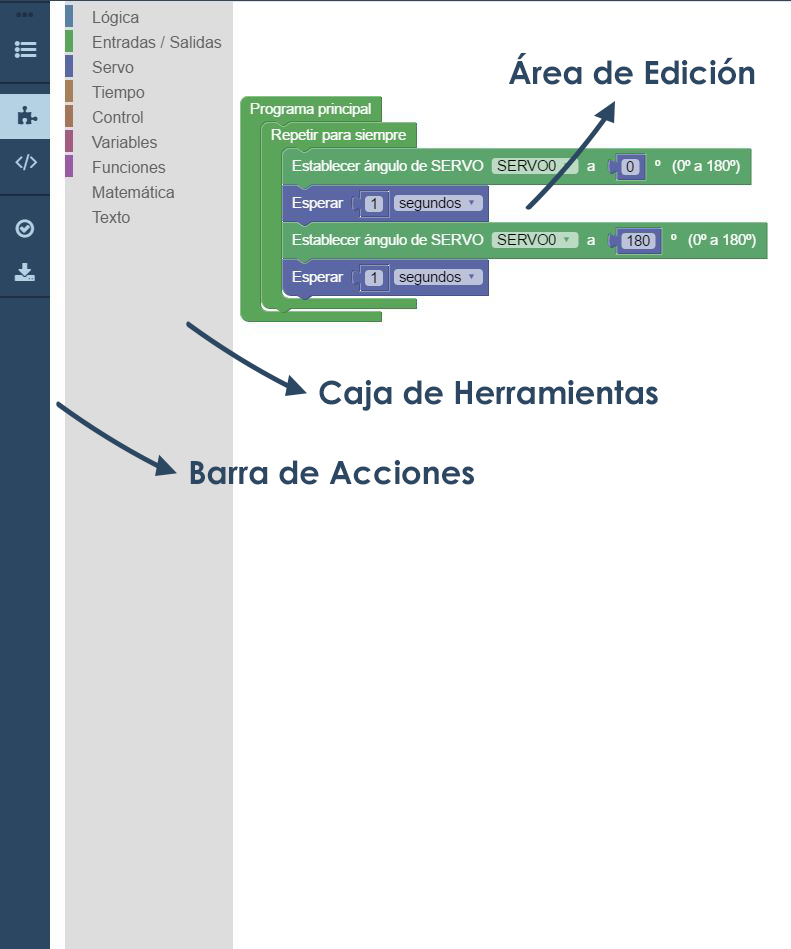
\includegraphics[scale=.50]{./Figures/editor.jpg}
	\caption{Área de flujo de trabajo de CIAABOT-IDE. Recuperado de \url{https://laboratorios.fi.uba.ar}}
	\label{fig:editor}
\end{figure}

\subsection{\emph{Debug} y \emph{Debugger}}
\label{Debug y Debugger}

La depuración es un programa que ejecuta ciertas rutinas de código de otros programas (programa objetivo), con el fin de encontrar y eliminar errores de ejecución. Esta técnica permite al código ser examinado obteniendo información muy importante sobre el estado en el que se está ejecutando.

Mediante el proceso de depuración de programas, se puede identificar y corregir errores propios de programación, corriendo un programa paso a paso depurando
el código, parandolo o pausandolo, de esta manera se realiza el seguimiento de
valores de las variables críticas, dando en consecuencia la posibilidad al programador
de corregir errores y pulir el funcionamiento.

Como el software en general y los sistemas electrónicos se vuelven generalmente
más complejos, se da importancia al desarrollo de técnicas y herramientas de depuración,
precisamente por las ventajas que tiene, como son el detectar anomalías
en cada paso, corregir y mejorar las funcionalidades. 

La mayoría de las computadoras modernos tienen el soporte de su hardware para
realizar la depuración, en el caso de la EDU-CIAA-NXP cuenta con un puerto USB
para realizar la depuración de un programa en el microcontrolador. El \emph{debugger}
utilizado en el IDE-Eclipse puede realizar la depuración conectándose al puerto
USB.

La plataforma CIAABOT no posee ninguna forma que permita \emph{debuggear} un programa.
Para realizar los ensayos se tiene que compilar el programa, descargalo y luego manualmente probar la lógica en la placa usando, como por ejemplo, los leds, botones, mensajes por UART, etc.


%----------------------------------------------------------------------------------------

\section{Motivación}
\label{Motivación}

Se plantea el desarrollo de un \emph{debugger} interactivo para CIAABOT, debido a la
importancia de realizar pruebas de un programa en tiempo real, y de esta manera verificar la lógica del programa.

La importancia de usar un \emph{debugger} a nivel de bloques, es que permite al usuario
ir ejecutar las rutinas de código de manera mas pausada, ademas de ir monitoreando
el estado de las variables que son parte de su programa, ayudándolos a
identificar y subsanar los errores de ejecución.

El desarrollo del \emph{debugger} interactivo para CIAABOT, seguirá los lineamientos
de diseño de CIAABOT, implementando el desarrollo con una visión de
fácil utilización, simple e intuitivo, teniendo en cuenta quienes serán los usuarios
finales.

Se aprovechará con el desarrollo de esta implementacion poder aplicar todos los
conocimientos aprendidos durante la carrera de especialización de sistemas embebidos.


%----------------------------------------------------------------------------------------

\section{Objetivos y alcance}
\label{Objetivos y alcance}

El objetivo de este proyecto es brindarle al usuario una herramienta útil para la
corrección e identificación de los errores de programación cuando está usando
la plataforma CIAABOT. Para lograrlo se pretende desarrollar un \emph{debugger} para
CIAABOT que cumpla con las siguientes características: 

\begin{itemize}
	\item Ejecutar un programa línea a línea.
	\item Detener la ejecución temporalmente en un bloque encastrable concreto.
	\item Visualizar el contenido de las variables en un determinado momento de la
	ejecución.
	\item Entorno gráfico amigable, tooltips con valores sobre el código.
	\item Importar el programa de bloques creado en el IDE de desarrollo de CIAABOT.	
\end{itemize}

De esta manera el aprendizaje del usuario programador primerizo será didáctica,
identificando y subsanando los errores de ejecución.

%----------------------------------------------------------------------------------------







\chapter{Introducción Específica} % Main chapter title

\label{Chapter2}

%----------------------------------------------------------------------------------------
%	SECTION 1
%----------------------------------------------------------------------------------------
En este capítulo se presenta los componentes de CIAABOT, con un poco más
de detalle, se analiza una alternativa real para depuración y se justifica el diseño
propuesto de \emph{debugging} a implementar, luego se establecen los requerimientos y
la planificación para el desarrollo del presente trabajo.

\section{Componentes CIAABOT}
\label{sec:Componentes CIAABOT}
La plataforma esta conformada por tres partes fundamentales, tal como se muestra en la figura \ref{fig:componentesCiaabot}. 

A continuación se describirá en detalle cada una de las partes de CIAABOT.

\begin{figure}[h]
	\centering
	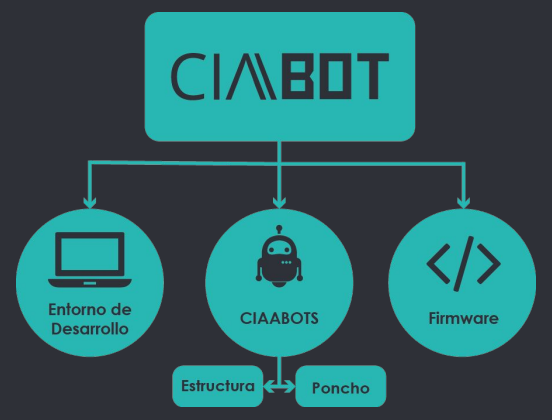
\includegraphics[scale=.50]{./Figures/componentesCiabot.png}
	\caption{Componentes CIAABOT. Recuperado de \url{https://laboratorios.fi.uba.ar}}
	\label{fig:componentesCiaabot}
\end{figure}

\subsection{CIAABOT IDE}

El IDE esta basado en el paradigma reactivo que permite armar programas propios, que pueden ser programas puntuales como manejo de actuadores y motores
en un sistema embebido, así como también, un prototipado rápido.

El IDE de CIAABOT tiene como componente principal al editor, a partir de allí el usuario puede empezar a desarrollar su propio programa gráfico encastrando de manera fácil bloques predifinidos creado en lenguaje javascript, como se observa en la figura \ref{fig:ciaabot-ide-bloques} 

El entorno de desarrollo integrado está diseñado para crear programas de forma sencilla encastrando bloques gráficos. Asimismo, permite de manera gradual ir comprendiendo como realizar el mismo programa en lenguaje C, debido a que permite ver en tiempo real el código C generado mientras se van encastrando los bloques.

Dentro del entorno se brinda al usuario, una barra de herramientas con funcionalidades
para crear un nuevo programa, compilarlo, y realizar la descarga del
código en la placa conectándola por USB.

El IDE proporciona al usuario la opción de guardar el programa creado en un
archivo con extensión .cbp, el cual contiene toda la información del programa
creado, que podría ser utilizado posteriormente. 

\begin{figure}[h]
	\centering
	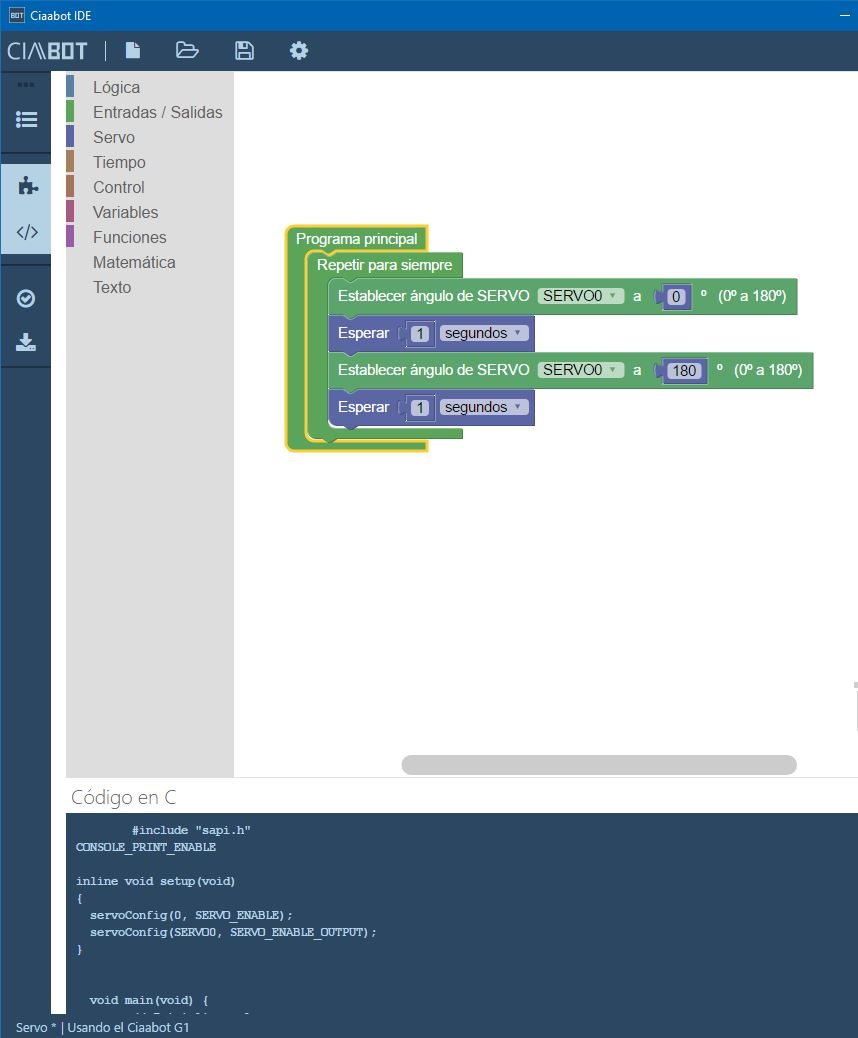
\includegraphics[scale=.30]{./Figures/ciaabot-ide-bloques.JPG}
	\caption{Editor gráfico de CIAABOT-IDE.}
	\label{fig:ciaabot-ide-bloques}
\end{figure}

La plataforma CIAABOT esta programado usando las siguientes tecnologías:

\begin{itemize}
	\item Angular\citep{angular}.
	\item Blockly\citep{blockly}.
	\item Electrón\citep{electron}.
	\item NodeJS\citep{nodejs}.
	\item TypeScript\citep{typescript}
\end{itemize}

El funcionamiento principal en la plataforma CIAABOT es la siguiente:

\begin{itemize}
	\item Genera el archivo principal: archivo main.c
	\item Genera el código en C: cada uno de los bloque genera el correspondiente codigo en C y lo inyecta en el archivo main.c del programa.
	\item Permite la ejecución del compilador de C para el código en la placa.
	Invoca al OpenOCD.
	\item Descarga el binario compilado en flash y realiza el reset.
\end{itemize}

\subsection{CIAABOTS}
\label{subsec:CIAABOTS}

La plataforma usa CIAABOTS para llamar así a los robots que se pueden programar utilizando CIAABOT IDE. Estos CIAABOTS tienen un diseño estructural de impresión en 3D, correspondiente al modelo de la placa CIAA. 

Para ser usados por las impresoras 3D, es necesario armar el poncho de diseño abierto y tener los sensores y actuadores del CIAABOT a imprimir.

\subsection{Firmware}
\label{subsec:Firmware}

Debido a que la plataforma CIAABOT esta basado en el firmware v2 \citep{CIAA:firmwarev2} del proyecto CIAA, puede crear desde funciones simples a más complejas, para realizarlo
utiliza las siguientes herramientas:

\begin{itemize}
	\item \emph{Makefile}: para la gestión de dependencias, de esta manera puede construir
	el software desde sus archivos fuente.	
	\item \emph{OpenOCD}: una herramienta OpenSource, usado para el grabado del firmware
	en las placas.
	\item \emph{sAPI}\citep{sAPI}: permite manejar los periféricos del microcontrolador de una manera
	muy sencilla.
\end{itemize}


\section{Alternativas de diseño para CIAABOT debugger}
\label{sec:Alternativas de diseño para CIAABOT debugger}

Para diseñar el software de depuración se toma como caso de estudio, la depuración de un programa en lenguaje C mediante Eclipse IDE:

\begin{itemize}
	\item \emph{Plugin de eclipse arm-none-eabi-gdb}
	\footnote{Software de configuración de eclipse para usar el depurador GNU para procesadores ARM Cortex-A/R/M.}: realiza la interpretación de comandos de	GDB-MI y muestra los resultados en la interfaz gráfica del editor de texto de C en el IDE del Eclipse.
	\item \emph{arm-none-eabi-gdb}
	\footnote{Software de debug originario de linux.}: realiza el mapeo de los símbolos de C con las instrucciones en código máquina que se ejecutan en el microcontrolador (mapea las funciones al código binario en flash), para
	luego ejecutar los comandos de parar, continuar o de uso de brakpoints. Se podría debuggear también, por línea de comandos directamente sobre el código C abriendo GDB en una terminal con comandos GDB-MI y usando los archivos .elf y .bin generados.
	\item \emph{OpenOCD (Open On-Chip Debugger)}\footnote{Software de código abierto que interactúa con el puerto JTAG de un depurador de hardware.}: prevee a GDB el remote interface protocol para permitirle acceder al hardware. Traduce transacciones JTAG o SWD (mediante el puerto serie sobre USB) a comandos remote-protocol de GDB. OpenOCD utiliza scripts de configuración (archivos *.cfg) donde se describe el microcontrolador a depurar y la interfaz de hardware para acceder al mismo (en adelante \emph{"Debugger HW"}).
	\item \emph{Debugger (HW)}: en el caso de la EDU-CIAA es la placa de interfaz fisica para pasar de JTAG a USB (modo puerto serie virtual). En la EDU-CIAA
	viene incluido en la misma placa que esta el micro y usa todo el circuito de hardware para debug.
	\item \emph{Microcontrolador a debuggear}: El microcontrolador posee un periferico específico para \emph{debug} con interfaz JTAG
	\footnote{Acrónimo de Joint Test Action Group, es utilizado como mecanismo para depuración de sistemas embebidos, proveendo una puerta trasera para acceder al sistema.}, teniendo acceso para modificar la RAM, Flash (externas al microcontrolador) y los registros del Microcontrolador.
\end{itemize}

Una alternativa para la programación de un software de depuración a nivel de bloques de CIAABOT es, entonces, mantener el mapeo entre los bloques de programa de CIAABOT y su C generado y comunicarse con GDB, mediante GDB-MI como lo realiza el plugin de Eclipse.

Teniendo en cuenta la complejidad de implementar lo visto anteriormente, se propone como una alternativa factible, el de emular la funcionalidad de debugger mediante la ejecución del programa de CIAABOT en la propia PC, de manera que al momento de ejecutarse los bloques gráficos de acceso a los periféricos, se realice la comunicación con la placa mediante un protocolo, y de esta manera realizar la ejecución de comandos de lectura y escritura en los periféricos que se quiere manipular.

Debido a que existe como antecedente el proyecto firmata4CIAA se decidió utilizarlo como protocolo para acceso al Hardware.


\section{Firmata}
\label{sec:Firmata}

Firmata es un protocolo genérico para comunicarse con microcontroladores desde
el software en una computadora (o teléfono inteligente / tableta, etc.).

Este protocolo fue diseñado para la comunicación directa entre un microcontrolador y un objeto de software en una computadora host Cliente Firmata. En la figura \ref{fig:componentesFirmata} se muestra la Arquitectura de este protocolo.

Firmata4CIAA es un programa que implementa el protocolo firmata en la EDU-CIAA-NXP.

\begin{figure}[h]
	\centering
	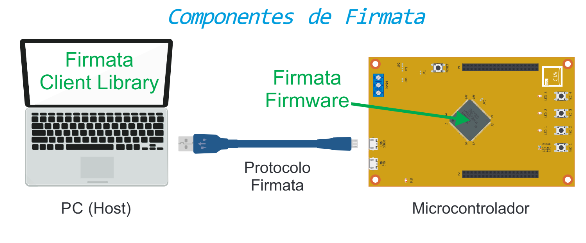
\includegraphics[scale=.80]{./Figures/componentesFirmata.png}
	\caption{Arquitectura de Firmata.}
	\label{fig:componentesFirmata}
\end{figure}

\subsection{Johnny-Five}
\label{subsec:Johnny-Five}

Cliente firmata, basado en el lenguaje JavaScript. Es un marco de programación de fuente
abierta, basado en el protocolo firmata, IoT y Robótica. En la figura \ref{fig:johnny} se presenta a este framework.

\begin{figure}[h]
	\centering
	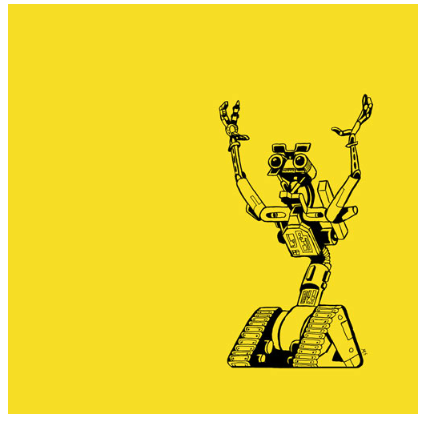
\includegraphics[scale=.50]{./Figures/johnny.png}
	\caption{Cliente firmata: Johnny-Five. Recuperado de \url{http//johnny-five.io}} 
	\label{fig:johnny}
\end{figure}

De esta manera se propone la comunicación entre la aplicación y la placa EDUCIAA-NXP.

\section{Sistema para depuración propuesto}

Después de lo visto en las secciones anteriores, se propone el siguiente sistema a diseñar:

\begin{itemize}
	\item Ejecutar un programa línea a línea, que ejecute los bloques en javascript en la PC del usuario..	
	\item Enviar comandos firmata a la placa, solo cuando se encuentre un bloque de acceso a algún periférico.
	\item Visualizar el contenido de las variables en un determinado momento de la ejecución.
	\item Instalación del protocolo firmata de la CIAA, sólo en el caso de ser necesario.
	\item Entorno gráfico amigable.
\end{itemize}

\subsection{Limitación}
\label{subsec:Limitación}

En este sistema propuesto, existen dos tipos de ejecución de bloques:

\begin{itemize}
	\item Bloques gráficos que acceden a los periféricos: son aquellos que usarán el protocolo firmata para enviar comandos a la placa, y mediante las funciones por UART se van comunicando con el hardware. Por ejemplo en el manejo de sensores, motores, etc.
	\item Bloques gráficos que no acceden a los periféricos: son aquellos que se ejecutan en la misma pc, por medio de javascript. Por ejemplo las sentencias loop-for, if-else, etc.
\end{itemize}

Los bloques gráficos que acceden a los periféricos, en tiempo de acceso de ejecución,
serán más lentos que si se tuviera que implentar la alternativa de diseño de
la sección \ref{sec:Alternativas de diseño para CIAABOT debugger}, ya que ese programa accedería al hardware a la velocidad en la que
se llama a las instrucciones del hardware, debido al código binario compilado
instalado en la placa.

Por el contrario, los bloques gráficos que no acceden a los periféricos, en tiempo
de ejecución, serán más rápidos, debido a que se ejecutarán directamente en la
misma PC del usuario. El programa se ejecutará dentro del contexto del VM de
javascript, que es más rápido que el código c compilado en el microcontrolador.

En conclusion si medimos los tiempos de ensayos, cuando se instala el firmware
del codigo C generado en la placa contra la ejecución de los bloques con firmata, estos tiempos no serán los mismos.

\subsection{Ventaja}
\label{subsec:Ventaja}

Para el usuario de CIAABOT, este método será una ventaja, ya que podrá depurar el programa sin necesidad de esperar la generación del código C a partir del programa en bloques, su compilación (especialmente en Windows) y descarga a la plataforma.

\section{Requerimientos}
\label{sec:ejemplo}

Se plantearon requerimientos que el proyecto debe cumplir a la hora de ser en-
tregado. Se evaluaron sus posibilidades y se clasificaron en categorías.

\subsection{Requerimientos asociados con el Proyecto CIAABOT}

\begin{itemize}
	\item El entorno de programación deberá poder ejecutarse minimamente dentro del entorno Linux y Windows.	
	\item El uso debe ser sencillo, rápido e intuitivo.
	\item El entorno de debugger debe tener un diseño basado en ventanas cómodas y que permitan
	tener mucha información a la vista.
	\item El entorno de debugger debe ocupar muy poca memoria.
	\item El diseño de la herramienta debe seguir los estilos de interfaz establecidos en el Proyecto CIAABOT.
	\item La herramienta debe poder permitir el monitoreo de las entradas y salidas de los diferentes periféricos de la placa.	
\end{itemize}

\subsection{Componentes establecidos en CIAABOT}

\begin{itemize}
	\item El presente proyecto deberá integrarse al entorno gráfico establecido que permita la programación de los robots.	
	\item Se usará la placa EDU-CIAA-NXP (figura \ref{fig:edu-ciaa-nxp}) para el control de los robots.	
\end{itemize}

\begin{figure}[h]
	\centering
	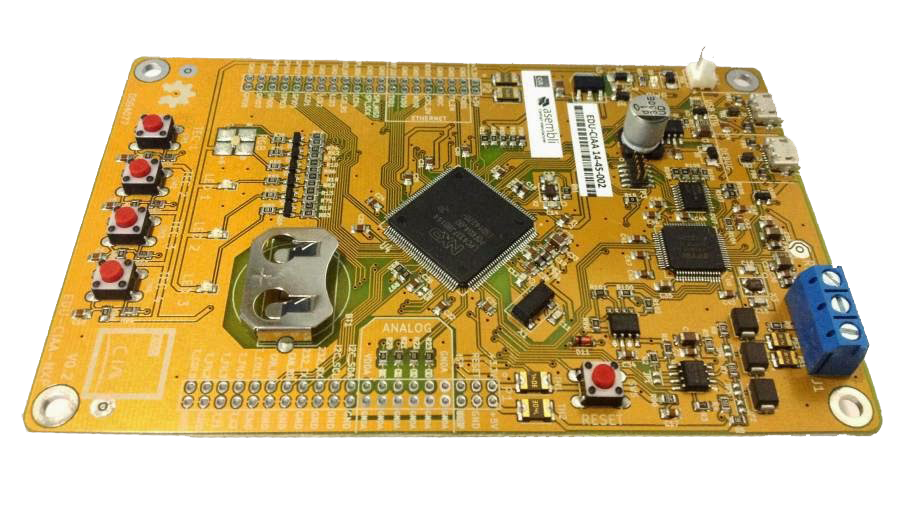
\includegraphics[scale=.30]{./Figures/edu-ciaa-nxp.png}
	\caption{Placa EDU-CIAA-NXP}
	\label{fig:edu-ciaa-nxp}
\end{figure}

\subsection{Firmware}

\begin{itemize}
	\item Se actualizará a la última versión, respetando el control de versiones establecido.	
	\item Se utilizarán las principales bibliotecas firmata que permita interactuar con el cliente que está corriendo en la placa.
	\item Se contará con un mecanismos de ahorro de la flash, para saber si la placa ya tiene firmata.
\end{itemize}

\subsection{Procesos Finales}

\begin{itemize}
	\item Se actualizará el manual de usuario, y se incluirán ejemplos básicos funcionales del entorno de depuración.	
	\item Se utilizarán las principales bibliotecas firmata que permita interactuar con el cliente que está corriendo en la placa.
	\item Se implementará el debugger de la aplicación sobre una maqueta o robot adaptado a funcionar con la placa EDU-CIAA.
	\item Se evaluarán los resultados del proyecto y su facilidad de uso en ámbitos de enseñanza reales.
\end{itemize}

\section{Planificación}
\label{sec:ejemplo}

Para lograr los objetivos propuestos, se realiza el desglose en tareas, y se utiliza las herramientas del diagrama de Activity on-node y gantt donde se esquematiza esas tareas que son parte del trabajo.

\subsection{Desglose en tareas} 

Para alcanzar objetivos concretos, se plantean los entragables para el proyecto:

\begin{itemize}
	\item Pluggin Debugger	
	\item Código fuente del proyecto debugger.
	\item Actualización del Manual de usuario, mostrando ejemplos didácticos del uso del debugger en la plataforma..
	\item El presente informe final.
\end{itemize}

Se estimó un tiempo aproximado de 600 horas, distribuidas en grupos de tareas de
la siguiente manera:

\begin{enumerate}
	\item Planificación del proyecto (60 hs.).
	
	\begin{itemize}
		\item Plan del proyecto.
		\item Análisis de requerimientos.
		\item Análisis técnico y de factibilidad.
		\item Gestión de riesgos.
		\item Gestión de calidad.
	\end{itemize}

	\item Investigación Preliminar (40 hs.).
	
	\begin{itemize}
		\item Búsqueda de plataformas de robótica educativa existentes, que en su interfaz de desarrollo implemente la herramienta de debugging.
		\item Búsqueda de frameworks de JavaScript, para la implementación de las funciones de firmata.
		\item Búsqueda de información acerca de la ejecución de debugging multiplataforma.
		\item Búsqueda de intérpretes Javascript para el debugging.
		\item Búsqueda de información de mecanismos de ahorro de la flash.
	\end{itemize}

	\item Selección de Frameworks (35 hs.).
	
	\begin{itemize}
		\item Selección y pruebas preliminares de la biblioteca firmata para JavaScript.
		\item Selección y pruebas preliminares del intérprete Javascript.
		\item Búsqueda de información acerca de la ejecución de debugging multiplataforma.
		\item Selección y pruebas del mecanismo de ahorro de la flash.
		\item Evaluar la correcta integración entre la aplicación CIAABOT y el debugger.
	\end{itemize}
	
	\item Desarrollo del Debugger (85 hs.).
	
	\begin{itemize}
		\item Desarrollo de estructura amigable e intuitiva para su uso.
		\item Desarrollo de estilos de componente compatibles a la aplicación CIAABOT.
		\item Desarrollo de módulo de configuración de mensajes al moverse los diferentes periféricos de la placa.
		\item Desarrollo del mecanismo de ahorro de la flash.
	\end{itemize}
	
	\item Implementaciones de funciones firmata javascript (90 hs.).
	
	\begin{itemize}
		\item Implementar los módulos para JavaScript encargados de obtener datos de cada sensor.
		\item Implementar los módulos para JavaScript encargados de manejar los actuadores.
		\item Desarrollo de funciones complementarias utilizando la API de JS Interpreter.
		\item Integración de las bibliotecas de programación gráfica.
	\end{itemize}

	\item Programación por Interfaz serie y Monitoreo Firmata (40 hs.).
	
	\begin{itemize}
		\item Desarrollo para mostrar mensajes en la interacción de los diferentes periféricos de la placa cuando está conectada por interfaz serie.
		\item Desarrollo de monitoreo en modo debug, de los estados de entradas y salidas a traves de firmata con visualización en la aplicación.
	\end{itemize}

	\item Pruebas de Firmware (60 hs.).
	
	\begin{itemize}
		\item Pruebas Unitarias.
		\item Pruebas de Integración.
		\item Corrección de errores encontrados.
	\end{itemize}

	\item Integración del Sistema (60 hs.).
	
	\begin{itemize}
		\item Integración de la aplicación Ciaabot para el modo debug.
		\item Pruebas iniciales de todo el sistema Ciaabot.
		\item Corrección de errores encontrados.
	\end{itemize}

	\item Procesos Finales (130 hs.).
	
	\begin{itemize}
		\item Modificar el manual de usuario, agregando el uso del modo debug.
		\item Redacción de memoria de trabajo.
		\item Evaluar el cumplimiento de requerimientos.
		\item Preparación de la presentación del proyecto.
	\end{itemize}

\end{enumerate}

\subsection{Activity On-node} 

En el diagrama de Activity on node de la figura  \ref{fig:diagramaNode} se muestran todas las tareas propuestas que se planificaron para realizar el proyecto, junto con su respectivo tiempo estimado en días para cada tarea.
Todas las flechas entrantes a un nodo o tarea son las dependencias de la misma.
 

\begin{figure}[h]
	\centering
	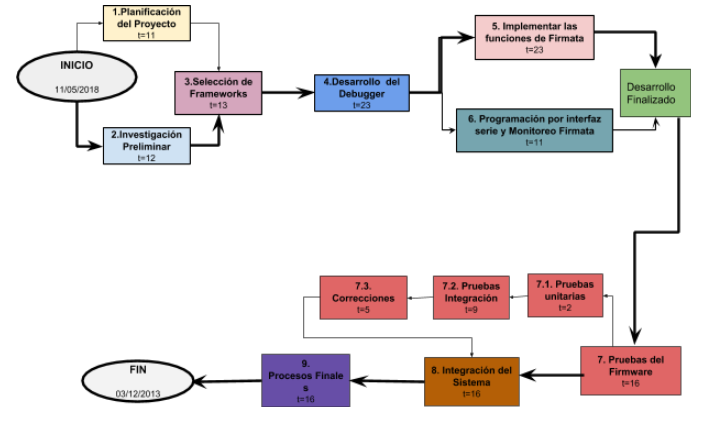
\includegraphics[scale=.60]{./Figures/diagramaNode.png}
	\caption{Diagrama de Node.}
	\label{fig:diagramaNode}
\end{figure}

Los días están expresados en días laborales de aproximadamente 3 horas, y en días no laborales de aproximadamente 4 horas. 
A modo de referencia se muestra en la siguiente figura  \ref{fig:tablaColores} una tabla de colores que se corresponde con cada una de las tareas.

\begin{figure}[h]
	\centering
	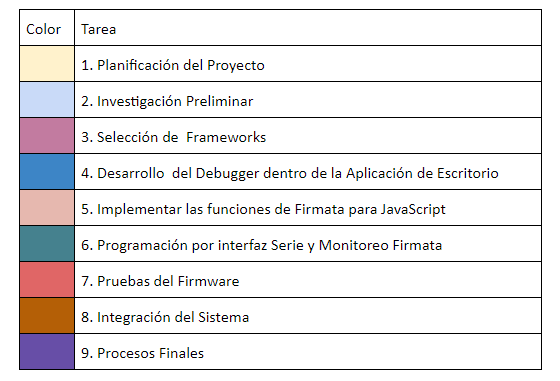
\includegraphics[scale=.60]{./Figures/tablaColores.png}
	\caption{Tabla de colores diagrama Activity}
	\label{fig:tablaColores}
\end{figure}

\subsection{Diagrama de Gantt}

El diagrama de Gantt permite tener una referencia rápida de dónde se debería encontrar el desarrollo del proyecto según la planificación inicial.
Por lo tanto, como parte de la planificación del proyecto, se definieron las tareas necesarias para completar el trabajo y se establecieron las relaciones de correlatividad entre ellas, teniendo en cuenta su duración. 

En la figura \ref{fig:diagramaGanttPrimeraParte} se puede observar la primera parte del diagrama para este proyecto. Las horas en la duración de cada una de las tareas están expresadas en días laborables y no laborables.

\begin{figure}[h]
	\centering
	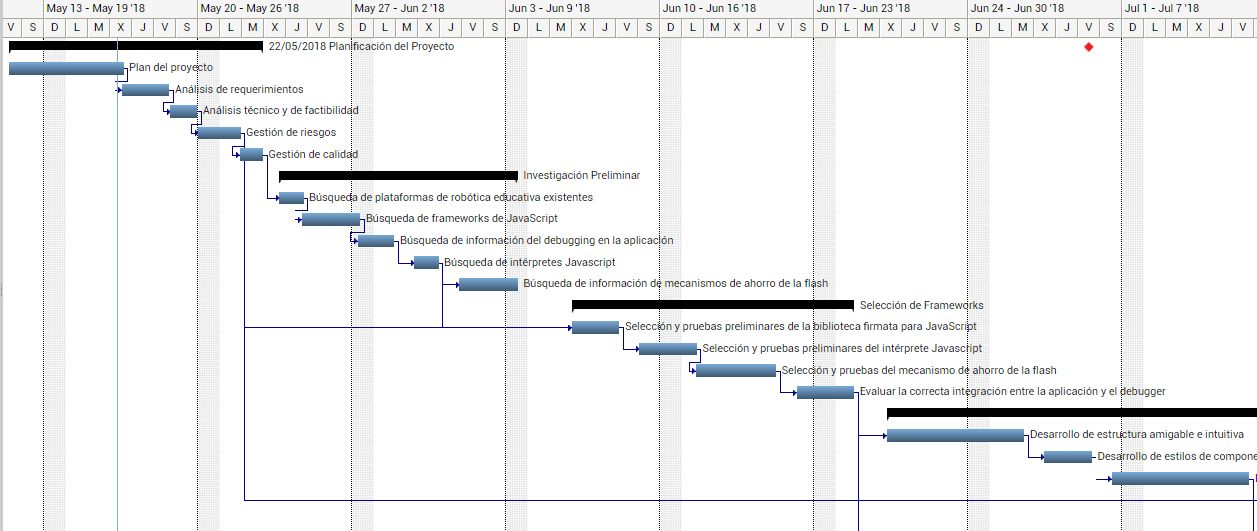
\includegraphics[scale=.30]{./Figures/diagramaGanttPrimeraParte.png}
	\caption{Diagrama de Gantt - Parte 1.}
	\label{fig:diagramaGanttPrimeraParte}
\end{figure}

En la figura \ref{fig:diagramaGanttSegundaParte} se puede observar la segunda parte del diagrama para este proyecto. 

\begin{figure}[h]
	\centering
	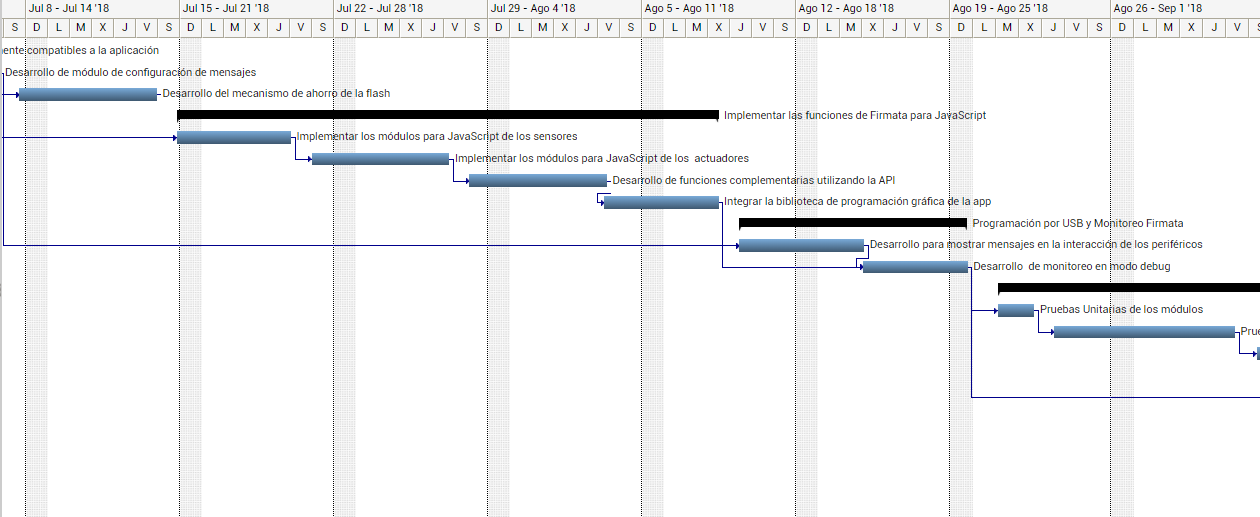
\includegraphics[scale=.30]{./Figures/diagramaGanttSegundaParte.png}
	\caption{Diagrama de Gantt - Parte 2.}
	\label{fig:diagramaGanttSegundaParte}
\end{figure}

En la figura \ref{fig:diagramaGanttTerceraParte} se puede observar la tercera parte del diagrama para este proyecto. Y la cuarta parte del diagrama se puede observar la figura \ref{fig:diagramaGanttCuartaParte} 

\begin{figure}[h]
	\centering
	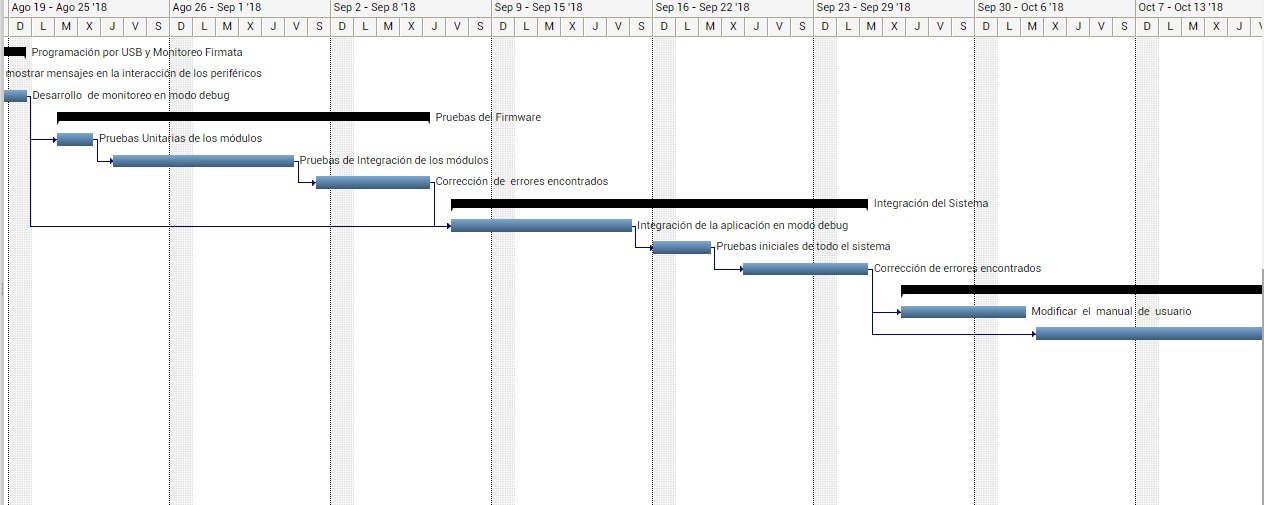
\includegraphics[scale=.30]{./Figures/diagramaGanttTerceraParte.png}
	\caption{Diagrama de Gantt - Parte 3.}
	\label{fig:diagramaGanttTerceraParte}
\end{figure}

\begin{figure}[h]
	\centering
	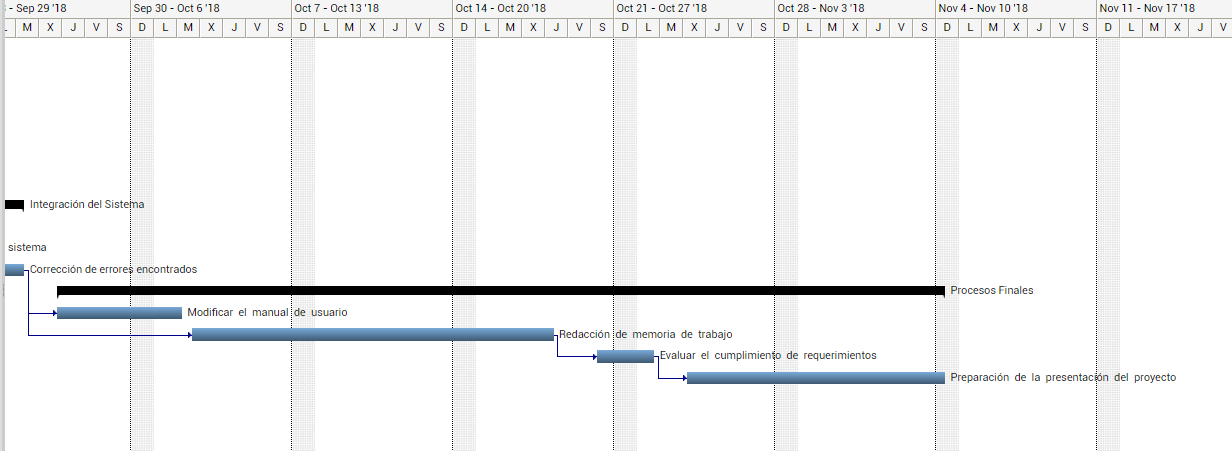
\includegraphics[scale=.30]{./Figures/diagramaGanttCuartaParte.png}
	\caption{Diagrama de Gantt - Parte 4.}
	\label{fig:diagramaGanttCuartaParte}
\end{figure}
 
\chapter{Diseño e Implementación} % Main chapter title

\label{Chapter3} % Change X to a consecutive number; for referencing this chapter elsewhere, use \ref{ChapterX}
\definecolor{mygreen}{rgb}{0,0.6,0}
\definecolor{mygray}{rgb}{0.5,0.5,0.5}
\definecolor{mymauve}{rgb}{0.58,0,0.82}

\lstset{ %
  backgroundcolor=\color{white},   % choose the background color; you must add \usepackage{color} or \usepackage{xcolor}
  basicstyle=\footnotesize,        % the size of the fonts that are used for the code
  breakatwhitespace=false,         % sets if automatic breaks should only happen at whitespace
  breaklines=true,                 % sets automatic line breaking
  captionpos=b,                    % sets the caption-position to bottom
  commentstyle=\color{mygreen},    % comment style
  deletekeywords={...},            % if you want to delete keywords from the given language
  %escapeinside={\%*}{*)},          % if you want to add LaTeX within your code
  %extendedchars=true,              % lets you use non-ASCII characters; for 8-bits encodings only, does not work with UTF-8
  %frame=single,	                   % adds a frame around the code
  keepspaces=true,                 % keeps spaces in text, useful for keeping indentation of code (possibly needs columns=flexible)
  keywordstyle=\color{blue},       % keyword style
  language=[ANSI]C,					% the language of the code
  %otherkeywords={*,...},           % if you want to add more keywords to the set
  numbers=left,                    % where to put the line-numbers; possible values are (none, left, right)
  numbersep=5pt,                   % how far the line-numbers are from the code
  numberstyle=\tiny\color{mygray}, % the style that is used for the line-numbers
  rulecolor=\color{black},         % if not set, the frame-color may be changed on line-breaks within not-black text (e.g. comments (green here))
  showspaces=false,                % show spaces everywhere adding particular underscores; it overrides 'showstringspaces'
  showstringspaces=false,          % underline spaces within strings only
  showtabs=false,                  % show tabs within strings adding particular underscores
  stepnumber=1,                    % the step between two line-numbers. If it's 1, each line will be numbered
  stringstyle=\color{mymauve},     % string literal style
  tabsize=2,	                   % sets default tabsize to 2 spaces
  title=\lstname,                   % show the filename of files included with \lstinputlisting; also try caption instead of title
  morecomment=[s]{/*}{*/}%
}

En este capítulo se presenta como caso de estudio el funcionamiento del software de depuración para programas en C mediante Eclipse IDE y se describe en detalle el desarrollo del diseño e implementación del sistema para depuración elegido. 

%----------------------------------------------------------------------------------------
%	SECTION 1
%----------------------------------------------------------------------------------------

\section{Descripción general}
\label{sec:Descripción general}

El sistema se compone de una computadora ejecutando la depuración de un programa en lenguaje CIAABOT, y la placa EDU-CIAA-NXP conectado a la computadora, por medio de una interfaz, desde donde el IDE del \emph{debug} realice la comunicación con el hardware como se muestra en la figura \ref{fig:pc-bloques}.

\begin{figure}[!htbp]
    \begin{center}  % [width=10cm,height=5cm] [width=\textwidth]
	\includegraphics*[width=10cm,height=5cm]{./Figures/pc-bloques.png}
	\par\caption{Modelo conceptual.}\label{fig:pc-bloques}
	\end{center}
\end{figure}


\section{Caso de estudio: depuración con eclipse}
\label{sec:Alternativa de diseño}

Para diseñar el software de depuración se toma como caso de estudio la depuración de programas escritos en lenguaje C con Eclipse IDE sobre la EDU-CIAA-NXP:

\begin{itemize}
	\item \emph{Plugin de eclipse arm-none-eabi-gdb}
	\footnote{Software de configuración de eclipse para usar el depurador GNU para procesadores ARM Cortex-A/R/M.}: realiza la interpretación de comandos de	GDB-MI y muestra los resultados en la interfaz gráfica del editor de texto de C en el IDE del Eclipse.
	\item \emph{arm-none-eabi-gdb}: software de debug originario de Linux que realiza el mapeo de los símbolos de C con las instrucciones en código máquina que se ejecutan en el microcontrolador (mapea las funciones al código binario en flash), para
	luego permitir ejecutar los comandos de parar, continuar o de uso de brakpoints.
	\item \emph{OpenOCD (Open On-Chip Debugger)}: software de código abierto que interactúa con el puerto JTAG de un depurador de hardware, provee a GDB el remote interface protocol para permitirle acceder al hardware. Traduce transacciones JTAG o SWD (mediante el puerto serie sobre USB) a comandos remote-protocol de GDB. OpenOCD utiliza scripts de configuración (archivos *.cfg) donde se describe el microcontrolador a depurar y la interfaz de hardware para acceder al mismo (en adelante \emph{"Debugger HW"}).
	\item \emph{Debugger HW}: en el caso de la EDU-CIAA es el circuito de interfaz fisica para pasar de JTAG a USB (modo puerto serie virtual). En la EDU-CIAA
	viene incluido en la misma placa que se encuentra el microcontrolador a depurar.
	\item \emph{Microcontrolador a depurar}: El microcontrolador posee un periferico específico para \emph{debug} con interfaz JTAG (Acrónimo de Joint Test Action Group, es utilizado como mecanismo para depuración de sistemas embebidos, proveendo una puerta trasera para acceder al sistema) teniendo acceso para modificar la RAM, Flash y los registros del Microcontrolador.
\end{itemize}

Una alternativa para la programación de un software de depuración a nivel de bloques de CIAABOT es, entonces, mantener el mapeo entre los bloques de programa de CIAABOT y su C generado, y comunicarse con GDB, mediante GDB-MI como lo realiza el plugin de Eclipse.

Teniendo en cuenta la complejidad de implementar lo expuesto, se propone como una alternativa factible, el de emular la funcionalidad de \emph{debugger} mediante la ejecución del programa de CIAABOT en la propia PC, de manera que al momento de ejecutarse los bloques gráficos de acceso a los periféricos, se realice la comunicación con la placa mediante un protocolo, para realizar la ejecución de comandos de lectura y escritura en los periféricos que se requiera manipular.

Como protocolo de comunicación para acceso al hardware se elije utilizar el protocolo firmata, debido a que existe una implementación del mismo para la EDU-CIAA-NXP \citep{CIAA:firmwarev2} y existen múltiples bibliotecas firmata para diferentes lenguajes de programación en la PC.  

\subsection{Firmata}
\label{subsec:Firmata}

Firmata es un protocolo genérico y abierto, fue diseñado para la comunicación directa entre un microcontrolador previamente instalado con un programa que implementa firmata y un objeto de software que implementa un cliente firmata en una computadora host. 

El protocolo se puede implementar en cualquier arquitectura de microcontroladores, así como en cualquier paquete de software.

Firmata4CIAA es un programa que implementa el protocolo firmata en la EDU-CIAA-NXP. En la figura \ref{fig:componentesFirmata} se muestra el uso de firmata con la EDU-CIAA-NXP.

\begin{figure}[h]
	\centering
	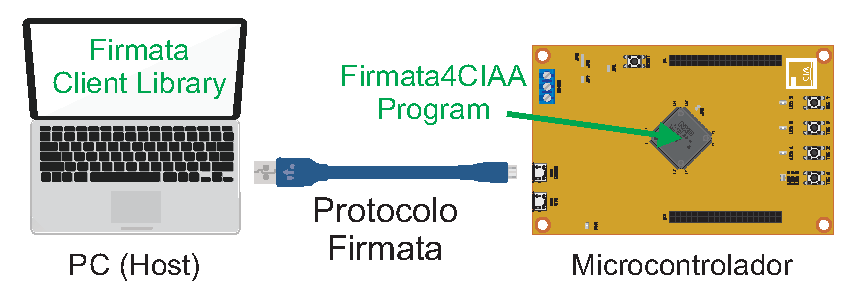
\includegraphics[scale=.80]{./Figures/Firmata4CIAA_01.pdf}
	\caption{Uso de firmata con la Educiaa.}
	\label{fig:componentesFirmata}
\end{figure}

\section{Sistema para depuración propuesto}
\label{section:Sistema para depuración propuesto}

El funcionamiento del entorno propuesto se puede resumir en los siguientes pasos:

\begin{itemize}
	\item Ejecutar un programa bloque a bloque en la PC, usando Javascript internamente, hasta que se encuentre con un bloque que requiera acceso a algún periférico del hardware.
	\item Enviar comandos firmata a la placa cuando se encuentre un bloque de acceso a algún periférico.
	\item Visualizar el contenido de las variables en un determinado momento de la ejecución.
	\item Instalación del programa que implementa el protocolo firmata en la EDU-CIAA-NXP, sólo en el caso de ser necesario.
\end{itemize}	

Cabe destacar que los bloques gráficos que acceden a los periféricos,
serán más lentos que si se tuviera que implementar mediante GDB-MI, ya que ese programa accedería al hardware a la velocidad en la que
se llama a las instrucciones del hardware, debido al código binario compilado
instalado en la placa.

Por el contrario, los bloques gráficos que no acceden a los periféricos, en tiempo
de ejecución, serán más rápidos, debido a que se ejecutarán directamente en la
misma PC del usuario. El programa se ejecutará dentro del contexto de la máquina virtual de
JavaScript, que es más rápido que el código C compilado en el microcontrolador.

De esta manera si se miden los tiempos de ensayos, cuando se instala el firmware
del código C generado en la placa contra la ejecución de los bloques con firmata, estos tiempos no serán los mismos.

Una ventaja para el usuario de CIAABOT, es que podrá depurar el programa sin necesidad de esperar el tiempo de compilación del código C generado a partir del programa en bloques (especialmente en Windows) y descarga a la plataforma reduciendo los tiempos de desarrollo del programa.


\section{Características del entorno \emph{CIAABOT Debug}}
\label{sec:Características del entorno CIAABOT debug}

El Entorno de Programación de \emph{CIAABOT Debug} debe ser capaz de permitirle al usuario realizar las siguientes tareas:

\begin{itemize}
	\item Abrir o importar un programa realizado en CIAABOT IDE.
	\item Ejecutar un programa bloque a bloque.	
	\item Establecer puntos de interrupción  (puntos de parada en los bloques).
	\item Permitir la visualización del valor de las variables durante la ejecución del programa.
	\item Ejecución del programa con o sin puntos de interrupciones activos (\emph{breakpoints}).
	\item Pausar y parar la ejecución del programa desde cualquier momento dado.
	\item Descarga del programa que implementa el protocolo firmata en la EDU-CIAA-NXP, sólo en el caso de ser necesario.
\end{itemize}

Los proyectos creados en CIAABOT IDE son guardados como archivos con extensión .cbp, la misma contiene la información del proyecto, su nombre, el modelo de CIAABOT utilizado
y el diagrama en bloques. Un proyecto puede abrirse desde el entorno de \emph{debug}, la información del proyecto es cargada y el diagrama en bloques es mostrado.

\section{Interfaz gráfica de \emph{CIAABOT Debug}}
La figura \ref{fig:debug-modos} expone el diseño realizado para la interfaz gráfica de \emph{CIAABOT Debug}.


\begin{figure}[!htbp]
	\begin{center}  % [width=10cm,height=5cm] [width=\textwidth]
		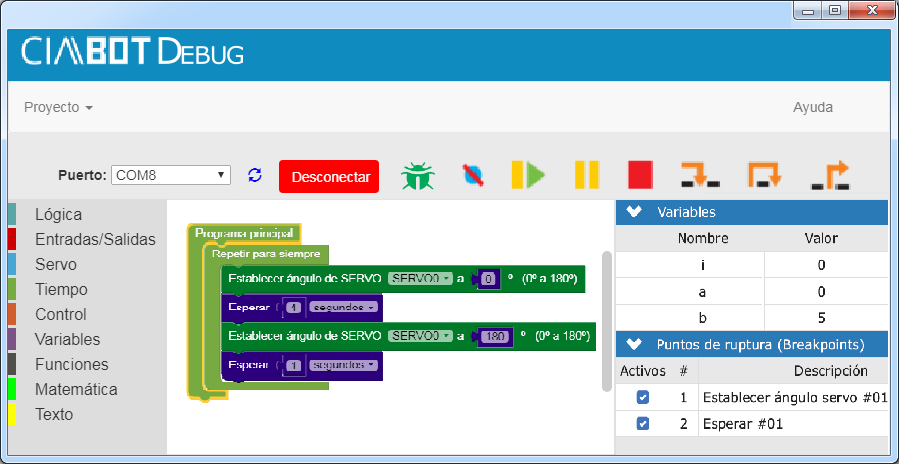
\includegraphics[width=15cm]{./Figures/CIAABOT-DEBUG-GUI-2.png}
		\par\caption{Diseño de la intergaz gráfica de \emph{CIAABOT Debug}.}\label{fig:debug-modos}
	\end{center}
\end{figure}


\emph{CIAABOT Debug} se compone de las siguientes partes:

\begin{itemize}
\item
Conexión con la plataforma.
\item
Editor de programa.	
\item
Iniciar sesión de depuración.
\item
Herramientas de control de ejecución.
\item
Menú de visualización de variables y puntos de interrupción.
\end{itemize}

En la figura \ref{fig:debug-modos} se resaltan cada una de ellas:

\begin{figure}[!htbp]
	\begin{center}  % [width=10cm,height=5cm] [width=\textwidth]
		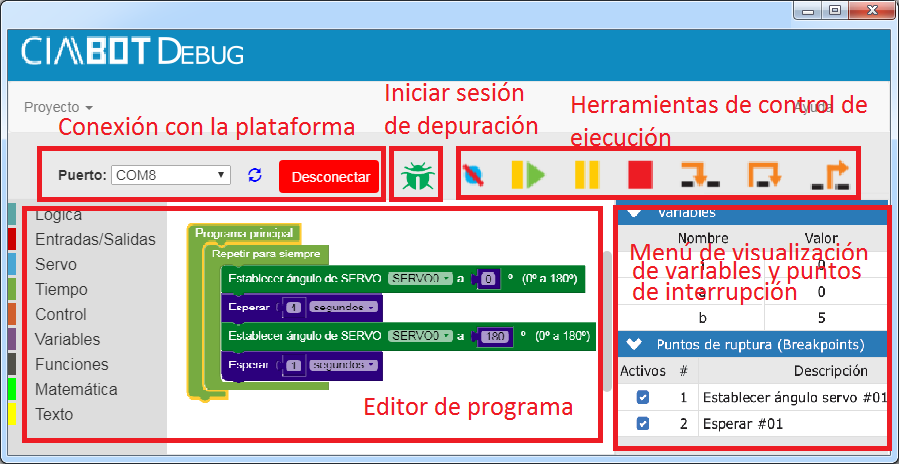
\includegraphics[width=15cm]{./Figures/CIAABOT-DEBUG-GUI-3.png}
		\par\caption{Composición de la intergaz gráfica de \emph{CIAABOT Debug}.}\label{fig:debug-modos}
	\end{center}
\end{figure}


\section{Máquina de estados de \emph{CIAABOT Debug}}
\label{sec:Modos de funcionamiento}

En la figura \ref{fig:diagrama-estados} se expone el diagrama de estados del software \emph{CIAABOT Debug}.


\begin{figure}[!htbp]
	\begin{center}  % [width=10cm,height=5cm] [width=\textwidth]
		\includegraphics*[width=15cm]{./Figures/diagrama-estados.pdf}
		\par\caption{Diagrama de máquina de estados de los modos de funcionamiento.}\label{fig:diagrama-estados}
	\end{center}
\end{figure}


\subsection{Desconectado}
\label{subsec:No Conectado}

La aplicación inicia en estado \emph{Desconectado}. En este modo de funcionamiento se permite la edición de bloques de programa, el botón de inicio de sesión de depuración se encuentra deshabilitado, así como las herramientas de control de ejecución. Mientras no este depurando se habilita la edición del programa. La figura \ref{fig:desconectado} expone la interfaz gráfica en este estado.


\begin{figure}[!htbp]
	\begin{center}  % [width=10cm,height=5cm] [width=\textwidth]
		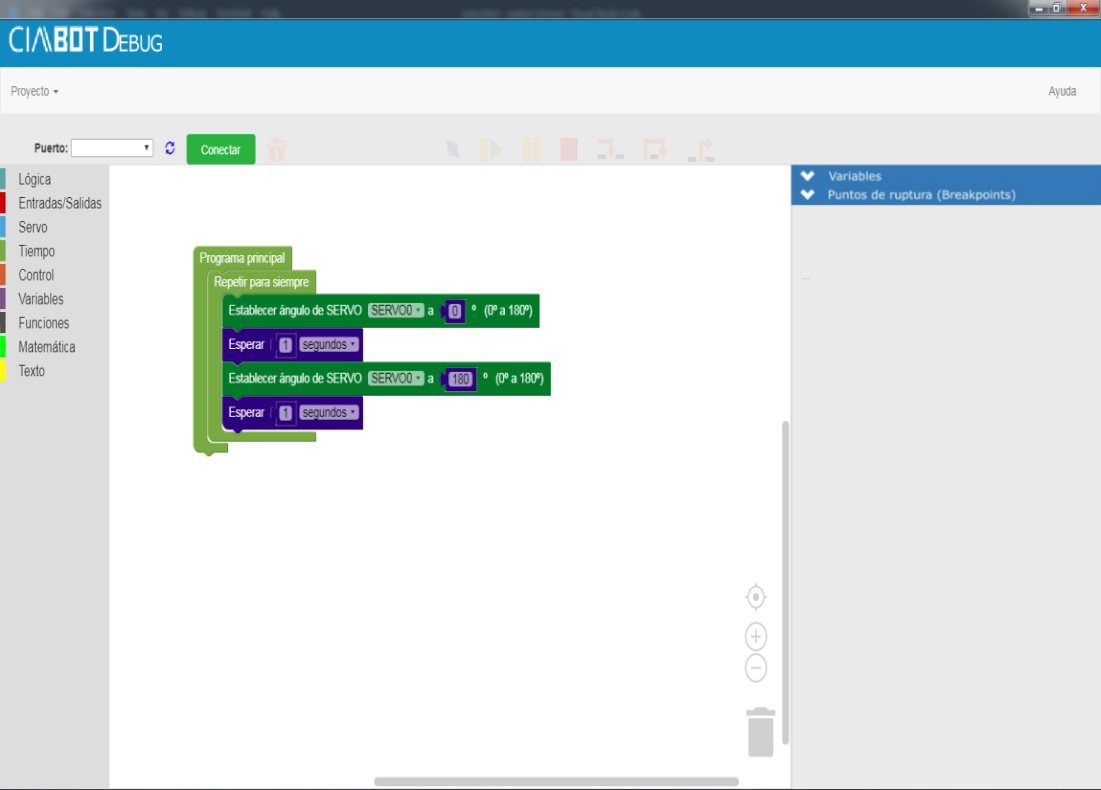
\includegraphics[width=15cm]{./Figures/debug-inicio.png}
		\par\caption{Estado Desconectado.}\label{fig:desconectado}
	\end{center}
\end{figure}


\subsection{Conectando}
\label{subsec:Conectando}

Cuando se presiona el botón “\emph{Conectar}” pasa al estado \emph{Conectando}. En este estado se permite la edición de bloques de programa y verifica si la EDU-CIAA-NXP tiene descargado el programa Firmata4CIAA, si lo tiene pasa a estado \emph{Conectado Con Firmata4CIAA}, sino pasa a \emph{Conectado Sin Firmata4CIAA}.

\subsection{Conectado Sin Firmata4CIAA}
\label{subsec:Conectado Sin Firmata4CIAA}

Si la aplicación paso a estado \emph{Conectado Sin Firmata4CIAA}, realiza la consulta al usuario si quiere descargar el programa Firmata4CIAA, si el usuario elige que sí, entonces se procede a realizar la descarga, y si elige que no entonces la aplicación vuelve al estado \emph{Desconectado}.

En la figura \ref{fig:instalar-firmata} muestra la consulta enviada al usuario.

\begin{figure}[!htbp]
	\begin{center}  % [width=10cm,height=5cm] [width=\textwidth]
		\includegraphics*[width=15cm]{./Figures/instalar-firmata.png}
		\par\caption{Descargar Firmata4CIAA.}\label{fig:instalar-firmata}
	\end{center}
\end{figure}

\subsection{Descargando Firmata4CIAA}
\label{subsec:Descargando Firmata4CIAA}

Firmata4CIAA, la aplicación pasa al estado \emph{Descargando Firmata4CIAA}. Si en medio del proceso existiese algún problema de descarga, se informará al usuario y volverá a estado \emph{Desconectado}.

Entre los archivos de \emph{CIAABOT Debug} se encuentra el proyecto de Firmata4CIAA previamente compilado para la EDU-CIAA-NXP. Para descargarlo el entorno requiere configurar la ruta del \emph{toolchain} y de \emph{OpenOCD}. Con esa información simplemente ejecuta el comando \emph{make download} en la ruta de dicho proyecto.

La figura \ref{fig:Configuracion} muestra la ventana desde donde se puede realizar la configuración de paths.

\begin{figure}[!htbp]
	\begin{center}  % [width=10cm,height=5cm] [width=\textwidth]
		\includegraphics*[width=12cm]{./Figures/Configuracion.PNG}
		\par\caption{Configuración de paths.}\label{fig:Configuracion}
	\end{center}
\end{figure}


\subsection{Conectado Con Firmata4CIAA}
\label{subsec:Conectado Con Firmata4CIAA}

En caso de que la conexión resulte exitosa y se compruebe la disponibilidad de Firmata en la plataforma, la aplicación pasa al estado \emph{Conectado Con Firmata4CIAA}, se habilita el inicio de sesión de depuración
En la figura \ref{fig:conectado} se muestra este modo de funcionamiento.


\begin{figure}[!htbp]
	\begin{center}  % [width=10cm,height=5cm] [width=\textwidth]
		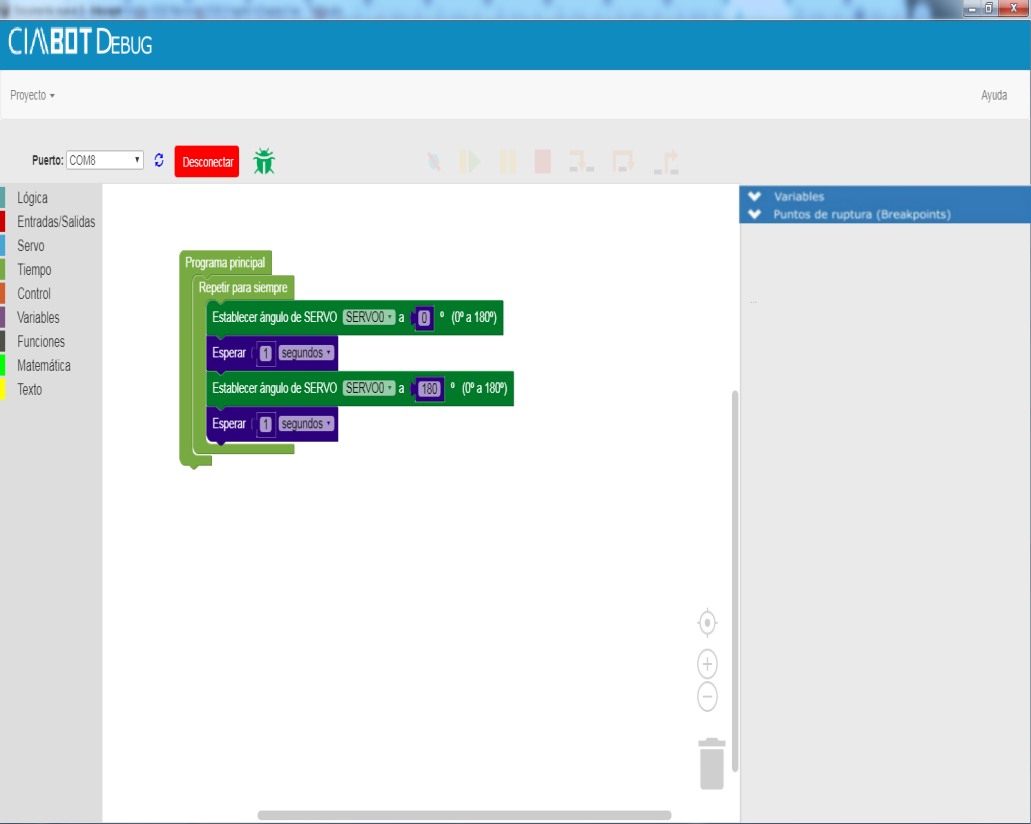
\includegraphics[width=15cm]{./Figures/debug-conectado.png}
		\par\caption{Estado Conectado con Firmata4CIAA.}\label{fig:conectado}
	\end{center}
\end{figure}

\subsection{Conectado En Sesión De Depuración}
\label{subsec:Conectado En Sesion De Depuración}

Si en el estado Conectado el usuario inicia la sesión de depuración, el entorno pasa a estado \emph{Conectado En Sesión de Depuración}. En este estado habilita la barra de herramientas de control de ejecución, permitiendole realizar el ensayo de su programa y deshabilita el menú de edición. La figura \ref{fig:debug} muestra la aplicación con este estado.

\begin{figure}[!htbp]
	\begin{center}  % [width=10cm,height=5cm] [width=\textwidth]
		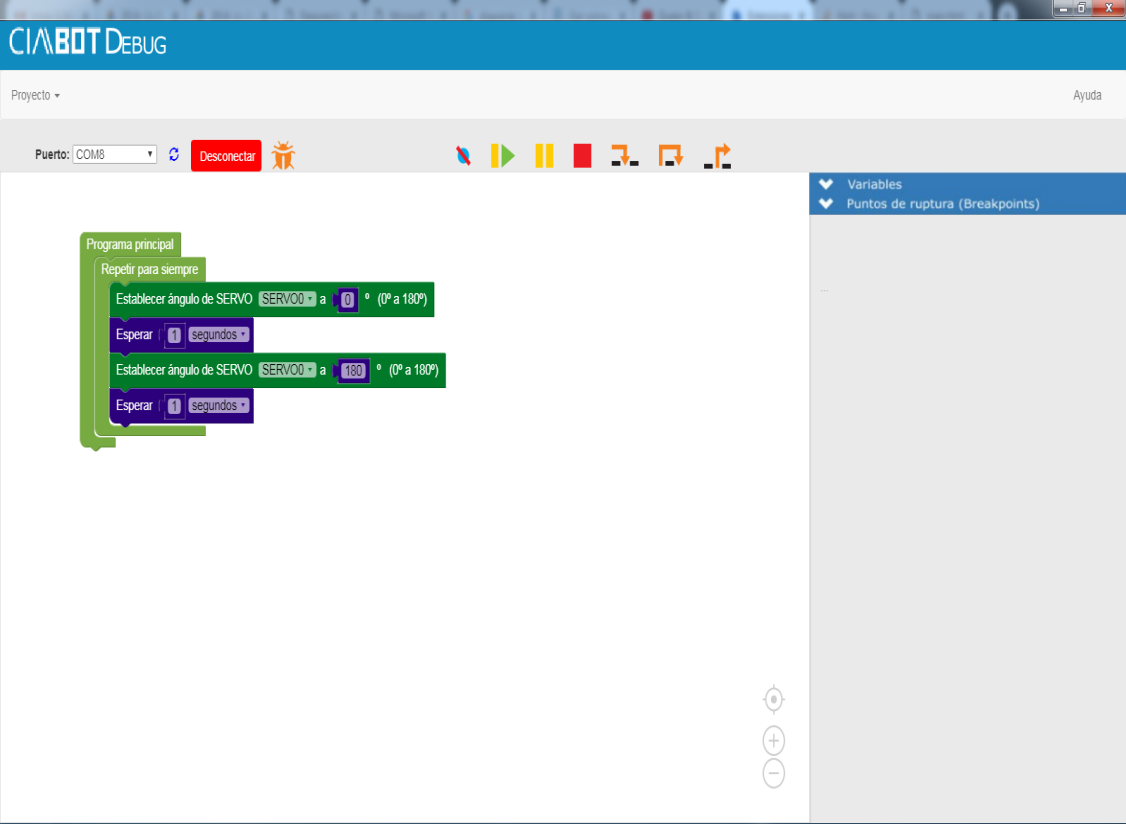
\includegraphics[width=15cm]{./Figures/debug-debug.png}
		\par\caption{Estado Depurando.}\label{fig:debug}
	\end{center}
\end{figure}


\section{Sesión de depuración}
\label{sec:Sesión de depuración}

\subsection{Iniciar/detener sesión}
\label{subsec:Iniciar/detener sesión}

Cuando inicia la aplicación el icono de \emph{debug} se muestra deshabilitado (color gris), como se muestra en la figura \ref{fig:debug_view_habilitada}.
Al tener la EDU-CIAA-NXP con Firmata4CIAA, la aplicación estará lista para iniciar la sesión de depuración, cambiando el icono de \emph{debug} de color gris (deshabilitado) a color verde (habilitado), de esta manera se permite al usuario mediante un click en el mismo, comenzar con la sesión de depuración. Al presionarlo, el botón se pone en color naranja, indicando que se ha iniciado una sesión de depuración y se deshabilita la acción de click sobre el mismo. Con la sesión de depuración iniciada el entorno habilita las herramientas de control de ejecución como se muestra en la figura \ref{fig:herramientas-control-ejecucion}.

\begin{figure}[h]
	\centering
	
\includegraphics[width=8cm]{./Figures/estadosBotonDebug.PNG}
	\caption{Estados del botón de depuración.}
	\label{fig:debug_view_habilitada}
\end{figure}


\begin{figure}[h]
	\centering
	
\includegraphics[width=10cm]{./Figures/herramientas-control-ejecucion.PNG}
	\caption{Herramientas de control de ejecución habilitada.}
	\label{fig:herramientas-control-ejecucion}
\end{figure}

La sesión de depuración finaliza cuando el usuario presiona el botón \emph{Detener depuración}, o si se cierra el programa en la aplicación.

\subsection{Herramientas de control de ejecución}
\label{subsubsec:Iniciar/Herramientas de control de ejecución}

En la tabla \ref{tabla:Comandos} se listan los botones de control de ejecución junto a una breve descripción.

\begin{table}[!htbp]
	\centering
	\begin{tabular}{ >{\centering\arraybackslash}m{2cm} >{\arraybackslash}m{2cm} >{\arraybackslash}m{7cm}}
		\hline
		Comando &  Nombre & Descripción \\
		\hline \hline
		
\includegraphics{./Figures/skip_breakpoints.PNG} & 
		Desactivar puntos de interrupción & Establece todos los puntos de interrupción para ser omitidos (Saltar todos los \emph{breakpoints}). \\
		\hline
		
\includegraphics{./Figures/resume.PNG} & 
		Ejecutar & Ejecuta el programa y Reanuda el programa si fue suspendido \\
		\hline
		
\includegraphics{./Figures/suspend.PNG} & Suspender & 
		Pausa el programa con el objetivo de que se pueda examinar, inspeccionar datos, pasos, etc. \\
		\hline
		
\includegraphics{./Figures/terminate.PNG} & Detener depuración & 
		Termina la depuración del programa. \\
		\hline
		
\includegraphics{./Figures/step_into.PNG} & Pasar adentro (\emph{step into}) & Ingresar a ejecutar el código en caso de ejecutar un llamado a función. \\
		\hline
		
\includegraphics{./Figures/step_over.PNG} & Pasar por encima (\emph{step over})& Continuar con el siguiente paso. La ejecución continuará en el siguiente bloque. En caso de que el bloque sea un llamado a función ejecutarlo sin ingresar al código de dicha función \\
		\hline
		
\includegraphics{./Figures/step_return.PNG} & Paso de regreso (\emph{step return}) & 
		Ejecutar hasta encontrar un retorno de función. \\
		\hline
	\end{tabular}
	\par\caption{Comandos de control de ejecución.}
	\label{tabla:Comandos}
\end{table}

El usuario podrá ejecutar un programa haciendo click en el ícono \emph{Ejecutar} de la barra de herramientas. De la misma manera para detener un programa en ejecución, podrá hacerlo mediante el icono \emph{detener ejecución}.

En la figura \ref{fig:debugPaso1} se expone un ejemplo de programa donde se ejecutan cada uno de los bloques con el comando  \emph{Pasar por encima (step over)}, comenzando por el bloque del programa principal, seguido por el bloque de repetir por siempre, y como siguiente paso, se muestra la ejecución de un bloque de establecimiento de un servomotor a 0 grados. En la figura \ref{fig:debugPaso2} se muestra la continuación del ejemplo anterior, en este paso se
muestra la ejecución de un bloque de espera de 1 segundo. Luego en la figura \ref{fig:debugPaso3} se
muestra la ejecución de un bloque de establecimiento de un servomotor a 180 grados.


\begin{figure}[!htbp]
	\begin{center}  % [width=10cm,height=5cm] [width=\textwidth]
		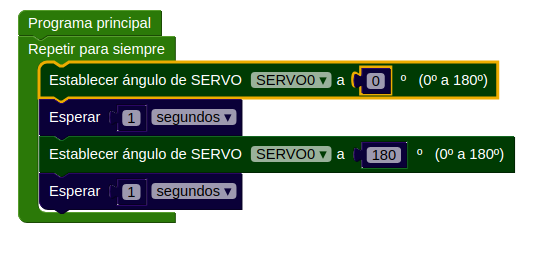
\includegraphics[width=12cm]{./Figures/debugPaso1.PNG}
		\par\caption{Resaltado del flujo de control (Parte 1).}\label{fig:debugPaso1}
	\end{center}
\end{figure}

\begin{figure}[!htbp]
	\begin{center}  % [width=10cm,height=5cm] [width=\textwidth]
		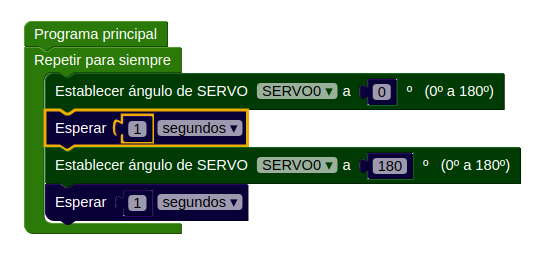
\includegraphics[width=12cm]{./Figures/debugPaso2.PNG}
		\par\caption{Resaltado del flujo de control (Parte 2).}\label{fig:debugPaso2}
	\end{center}
\end{figure}

\begin{figure}[!htbp]
	\begin{center}  % [width=10cm,height=5cm] [width=\textwidth]
		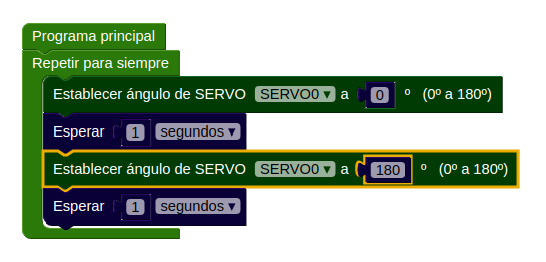
\includegraphics[width=12cm]{./Figures/debugPaso3.PNG}
		\par\caption{Resaltado del flujo de control (Parte 3).}\label{fig:debugPaso3}
	\end{center}
\end{figure}

La interfaz gráfica de usuario permite indicar al depurador cuándo pausar un programa, mediante el estableciendo de puntos de interrupción (\emph{breakpoints}).
Para establecer un de punto de interrupción, el entorno permite que el usuario haga click en el bloque en donde quiere pausar el programa. Cuando la ejecución del programa llege a este punto, el programa se detendrá. En la figura \ref{fig:add-breakpoint} se muestra el menú contextual del bloque desde donde se puede establecer el punto de interrupción.

\begin{figure}[!htbp]
	\centering
	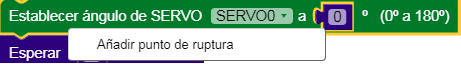
\includegraphics[width=10cm]{./Figures/add-breakpoint.PNG}
	\caption{Establecer una bandera de punto de interrupción.}
	\label{fig:add-breakpoint}
\end{figure}

Cuando se hace click en el bloque, debería mostrar un círculo rojo. Esto significa que el punto de interrupción se establece en ese bloque (figura \ref{fig:breakpoint}).

\begin{figure}[!htbp]
	\centering
	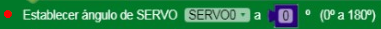
\includegraphics[width=10cm]{./Figures/breakpoint.PNG}
	\caption{Punto de interrupción.}
	\label{fig:breakpoint}
\end{figure}

Para eliminar el punto de interrupción del bloque, el usuario podrá removerlo desde el menú contextual del mismo bloque. Despues de realizar la acción, el circulo rojo del bloque se eliminará. Se ilustra el menú contextual en la figura \ref{fig:breakpoint-eliminar}.

\begin{figure}[!htbp]
	\centering
	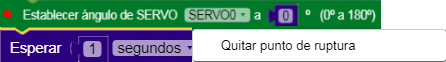
\includegraphics[width=10cm]{./Figures/breakpoint-eliminar.PNG}
	\caption{Quitar Punto de interrupción.}
	\label{fig:breakpoint-eliminar}
\end{figure}

Utilizando el botón \emph{Desactivar puntos de interrupción}, el entorno permite al alumno desactivar todos sus puntos de interrupción a la vez, sin eliminarlos, recordando cuales desactivo, entonces si se hace click nuevamente vuelven al estado original.
En la siguiente figura \ref{fig:desactivar-breakpoints} se muestra el ícono de este botón.

\begin{figure}[!htbp]
	\begin{center}  % [width=10cm,height=5cm] [width=\textwidth]
		
\includegraphics[scale=.90]{./Figures/desactivar-breakpoints.PNG}
		\par\caption{Desactivar los Puntos de interrupción activos.}\label{fig:desactivar-breakpoints}
	\end{center}
\end{figure}

\subsection{Menú de visualización}
\label{subsec:Iniciar/Menú de visualización}

El menú de visualización se divide en dos áreas, una para visualización de variables y otra para puntos de ruptura. La primera permite observar como cambian las variables de programa a medida que se ejecuta mientras está activa la sesión de depuración. En la siguiente figura \ref{fig:ventana-variables} se muestra el panel de variables.

\begin{figure}[!htbp]
	\centering
	\includegraphics*[width=9cm,height=3cm]{./Figures/variables.PNG}
	\caption{Menú de visualización de variables.}
	\par\label{fig:ventana-variables}
\end{figure}

La segunda, permite la visualización de todos los puntos de ruptura (\emph{breakpoints}) insertados en el programa, se permite modificar el estado activo/inactivo de cada punto de ruptura. En la siguiente figura \ref{fig:ventana} se muestra la ventana de \emph{breakpoints}.

\begin{figure}[!htbp]
	\centering
	\includegraphics*[width=8cm,height=2cm]{./Figures/breakpoints.PNG}
	\caption{Ventana de Puntos de ruptura (\emph{breakpoints}).}
	\par\label{fig:ventana}
\end{figure}

El entorno maneja la ejecución en los siguientes estados:

\begin{itemize}
	\item Ejecución de bloque sin breakpoint.
	\item Ejecución de bloque con breakpoints activos.	
	\item Ejecución de bloque con breakpoints inactivos.
\end{itemize}


\section{Edición de programa}
\label{sec:Edición de programa}

El área de edición de programa del entorno del \emph{debug}, contiene la misma estructura de bloques de la caja de herramientas de CIAABOT IDE, las cuales se dividen en las siguientes categorías:

\begin{itemize}
	\item Lógica.
	\item Entradas/Salidas.	
	\item Servo.
	\item Tiempo.
	\item Control.
	\item Variables.
	\item Funciones.
	\item Matemática.
	\item Texto.
\end{itemize}

El propósito, es permitir la modificación del programa cuando el usuario encuentre errores en la sesión de debug y quiera corregirlo en el entorno del \emph{debug}, de esta manera no tendrá la necesidad de guardar el programa para recién poder editarlo en CIAABOT IDE.


\section{Implementación}
\label{sec:Implementación}

\emph{CIAABOT Debug} esta desarrollado en el lenguaje Javascript. Permite importar un proyecto desde CIAABOT IDE con extensión .cbp y genera internamente código javascript para ejecutar la misma lógica que el programa en bloques. 
Para realizar esto se utiliza el archivo .cbp tiene la estructura de archivo de texto xml. Se separan los bloques gráficos que acceden a los periféricos de los bloques gráficos que no acceden a los periféricos, generando de esta manera el código correspondiente que integra todas las partes para que cuando se realice la ejecución del programa, lo haga de forma transparente para el usuario.

Mediante el cliente firmata Johnny-Five se establece la comunicación entre la aplicación y la placa EDU-CIAA-NXP, para el manejo de los periféricos. Johnny-Five es un cliente firmata, basado en el lenguaje javaScript, y dentro del entorno de \emph{debug}, es el encargado de interactuar con el microcontrolador con Firmata4CIAA para la manipulación de los periféricos.
En la siguiente figura \ref{fig:diagrama-bloques} se muestra el diágrama de bloques.

\begin{figure}[!htbp]
	\centering
	\includegraphics*[width=13cm]{./Figures/diagrama-bloques-2.PNG}
	\caption{Diágrama de Bloques para el manejo de los periféricos.}
	\par\label{fig:diagrama-bloques}
\end{figure}

\subsection{Implentación de la GUI}
\label{subsec:Implentación de la GUI}

A continuación se explicara las partes de bloques gráficos que ejecutan solo código javascript y las partes que ejecutan comandos de johnny five.

A modo de ejemplo, en la figura \ref{fig:codigo-servo-bloques} cómo se armaría en bloques el código para el barrido angular de un servomotor.

\begin{figure}[!htbp]
	\centering
	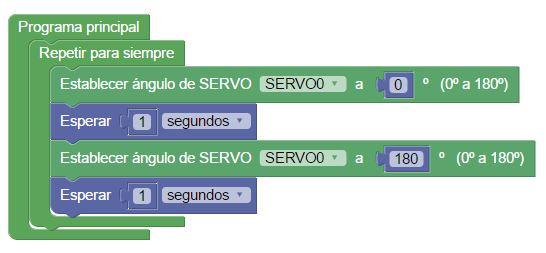
\includegraphics[width=12cm]{./Figures/ejemplo-servo.jpg}
	\caption{Ejemplo de código en bloques para el barrido de un servo.}
	\label{fig:codigo-servo-bloques}
\end{figure}

El código de salida en lenguaje Javascript de la figura \ref{fig:codigo-servo-bloques} se muestra 
en el Algoritmo 3.1:


\begin{lstlisting}[caption={Salida del código en bloques de la figura \ref{fig:codigo-servo-bloques}.}\label{cod:codigo-servo-c}] 
		                while(true){
			                	ciaa.setServo(0);
			                	wait.for(1, sec);
				                ciaa.setServo(180);
				                wait.for(1, sec);
		                };

\end{lstlisting}


\begin{itemize}
	\item Bloques gráficos que acceden a los periféricos: son aquellos que usarán el protocolo firmata para enviar comandos a la placa, y mediante las funciones por UART se van comunicando con el hardware. Por ejemplo en el manejo de sensores, motores, etc. En la figura \ref{fig:servoj5} se muestra un bloque de este tipo.
	
	
	\begin{figure}[!htbp]
		\centering
		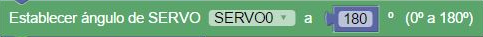
\includegraphics[width=12cm]{./Figures/ejemplo-servo-j5.PNG}
		\caption{Barrido de servomotor ejecutado con johnny five}
		\label{fig:servoj5}
	\end{figure}
   
    \begin{lstlisting}[caption={Código que ejecuta una de las funciones de johnny five del bloque de la figura \ref{fig:servoj5}.}\label{cod:codigo-servo-j5}] 
                  setServo: function(range) {
                    servo.to(range);
                  }
    \end{lstlisting}
	
	\item Bloques gráficos que no acceden a los periféricos: son aquellos que se ejecutan en la misma pc, por medio de javascript. Por ejemplo las sentencias loop-for, if-else, etc.  En la figura \ref{fig:waitj} se muestra un bloque de este tipo.
	
	\begin{figure}[!htbp]
		\centering
		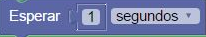
\includegraphics[width=6cm]{./Figures/ejemplo-servo-j.PNG}
		\caption{Ejemplo de wait}
		\label{fig:waitj}
	\end{figure}

	\begin{lstlisting}[caption={Código en javascript del bloque de la figura \ref{fig:waitj}.}\label{cod:codigo-servo-j}] 
			       for: function(time, unit) {
				        duration = time;
			        	waitStart = getTime(unit);
		           }
	\end{lstlisting}
\end{itemize}

En la figura \ref{fig:servoj5} se expone el bloque gráfico que utiliza los comandos de la API Johnny-five.io. A modo de ejemplo se hizo referencia a un bloque gráfico que usa la siguiente función: 

\emph{to(degrees 0-180 [, ms [, rate]])// establece la posición de 0 a 180 grados}


La figura \ref{fig:DocSecuencia} muestra el diagrama de secuencia del acceso a un periférico mediante el protocolo firmata.


\begin{figure}[!htbp]
	\begin{center}  % [width=10cm,height=5cm] [width=\textwidth]
		\includegraphics*[width=15cm]{./Figures/DocSecuencia.PNG}
		\par\caption{Diagrama de secuencia.}\label{fig:DocSecuencia}
	\end{center}
\end{figure}


\subsection{Herramientas utilizadas}
\label{subsec:Implementación del modelo computacional Servicios}

Para el desarrollo del entorno de \emph{debugger} se utilizaron los siguientes proyectos de código abierto:

\begin{itemize}
	\item Blockly \citep{blockly}: el lenguaje gráfico de CIAABOT IDE esta basado en esta biblioteca, por lo cual fue necesario la implementación de ciertas rutinas de código en javascript con la biblioteca blockly para lograr la visualización de los diagramas de bloques creados en CIABOOT IDE, así como también la manipulación de estos bloques gráficos para lograr la interacción con el interprete de Javascript. 
	
	\item Bootstrap \citep{bootstrap}: se uso esta biblioteca dentro de la aplicación para darle comportamiento a los botones del entorno del \emph{debug}, ya que provee todas las reglas CSS y HTML5 y se integra muy bien con las bibliotecas de javascript que usa el entorno.
	
	\item JS-Interpreter \citep{js-Interpreter}: el proyecto utiliza este intérprete de JavaScript ya que permite la ejecución línea por línea de código JavaScript generado para ejecutar el programas de usuario en bloques, y también para resaltar los bloques del programa a medida que se vayan ejecutando internamente. De esta manera los estudiantes podrán realizar un paso a través de su código para ver qué hace qué durante la depuración. 

	\item Acorn \citep{acorn}: es un rápido analizador tolerante a errores de JavaScript escrito en JavaScript, el analizador dentro del proyecto es usado para darle soporte al análisis/lectura de código del interprete de JavaScript.
	
	\item JQuery \citep{jQuery}: la biblioteca multiplataforma de JavaScript permite interactuar con los documentos HTML, manipular el árbol DOM de la página, agregar dinamismo a la aplicación y manejar eventos.
	
	\item Signals \citep{signals}: biblioteca escrita en JavaScript que implementa el patrón publicación/suscripción para agregar emisores de eventos al código cuando los bloques gráficos que se están ejecutando son resaltados.
	
	\item Johnny five \citep{johnny}: esta basado en Node.js y se integra muy bien con bibliotecas javascript que usamos en el entorno. Se utliza para la comunicación con la EDU-CIAA-NXP y trabajar con sus periféricos.
	
	\item Express \citep{express}: \emph{framework} de aplicación web ligero, rápido y muy útil, esta basado en http para Node.js, se usa para crear la aplicaciones web que luego son embebidas en una aplicación de escritorio. Esta biblioteca  proporciona funcionalidades como el enrutamiento, opciones para gestionar sesiones y cookies.
	
	\item Serialport \citep{serialport}: junto a firmata es usada para combinar JavaScript y hardware. Esta biblioteca permite el acceso a puertos series en la computadora.
	
	\item Electron \citep{electron}: permite armar el desarrollo de la aplicación de escritorio multiplataforma utilizando tecnologías web.
\end{itemize}


\subsection{Archivo de estado de \emph{CIAABOT Debug}}
\label{subsec:Archivo de CIAABOT Debug}

Cuando se abre un proyecto (archivo \emph{.cbp}), se crea un archivo \emph{.cbd} donde se guardan los puntos de interrupción que utiliza el usuario durante su sesión de depuración.

El archivo \emph{.cbd} se implementa mediante un archivo de texto en formato JSON \citep{json}. El mismo se guarda al cerrar el proyecto. De esta forma se recuperan los puntos de interrupción que fueron agregados al programa
y si se encuentran activos o no, de acuerdo a la elección realizada por el usuario en la última sesión de depuración. 

Si un proyecto luego es modificado por CIAABOT IDE, por ejemplo eliminando algún bloque que contenía un \emph{breakpoint}, al abrirlo nuevamente desde\emph{ CIAABOT Debug} se actualiza la información del archivo .cbd asociada al proyecto .cbp para mantener la coherencia entre los mismos.

Esta información es útil cuando el usuario cerro por algún motivo el entorno de \emph{CIAABOT Debug} y cuando lo vuelve a abrir no pierde el estado de los puntos de interrupciones utilizados en su última sesión de depuración.

En el Algoritmo 3.4 se expone un ejemplo de la estructura del archivo nombrado \emph{debug.cbd}.

\lstset{
	string=[s]{"}{"},
	stringstyle=\color{blue},
	comment=[l]{:},
	commentstyle=\color{black},
}

\begin{lstlisting}[caption={Estructura del archivo \emph{debug.cbd}} \label{cod:json}] 
{
  "type": "ciaabotDebugState",
  "breakpoins": [
     {
       "type": "asociation",
       "key": {
               "type": "logic_operation\",
               "id": "Ju6).aSXM}[dFL_Xw/p,\"
              },
       "value": {
                "type": "breakpoint",
                "id": 1,
                "active" : true
                }
     }, 
     {
       "type": "asociation",
       "key": {
               "type": "ciaa_sapi_gpio_digital_read",
               "id": "Oj7~RU|??CeufGPNV$|W\"
              },
       "value": {
                "type": "breakpoint",
                "id": 2,
                "active" : false
                }
      }
    ]
}
\end{lstlisting}


\subsection{GitLab}
\label{subsec:GitLab}

Como estrategia de mitigación del riesgo de pérdida de código, se propuso el versionado de código, para realizarlo se eligió la herramienta Gitlab, que es un servicio web de control de versiones y desarrollo de software colaborativo. Esta basado en Git y permite repositorios de código públicos y privados. 


% Chapter Template

\chapter{Ensayos y Resultados} % Main chapter title

\label{Chapter4} % Change X to a consecutive number; for referencing this chapter elsewhere, use \ref{ChapterX}

%----------------------------------------------------------------------------------------
%	SECTION 1
%----------------------------------------------------------------------------------------

Se realizaron pruebas funcionales sobre los requerimientos del proyecto.

\section{Ensayos preliminares sobre acerca del control de la plataforma mediante protocolo Firmata.}
\label{sec:Ensayos de control de la plataforma mediante protocolo Firmata}

Para comprobar el funcionamiento del entorno de depuración primero se comprobó mediante otro software el correcto acceso a la plataforma de hardware. Para esto se utilizó:

\begin{itemize}
	\item El programa \emph{Firmata test} \citep{firmataTest}, permite ensayar desde la PC el funcionamiento de una plataforma que soporte protocolo Firmata. La figura \ref{fig:firmataTest} expone la interfaz gráfica del software libre \emph{Firmata test}.
	\item La placa EDU-CIAA-NXP corriendo el programa Firmata4CIAA, el cual fue compilado y descargado de forma manual.
\end{itemize}

Se realizaron pruebas puntuales sobre los sensores y actuadores, demostrando el correcto acceso a todos los pines con sus respectivos modos de funcionamiento (los cuales pueden observarse en el Anexo I \ref{fig:MapeoPinesFirmata4CIAAv2}). 

\begin{figure}[!htbp]
	\centering
	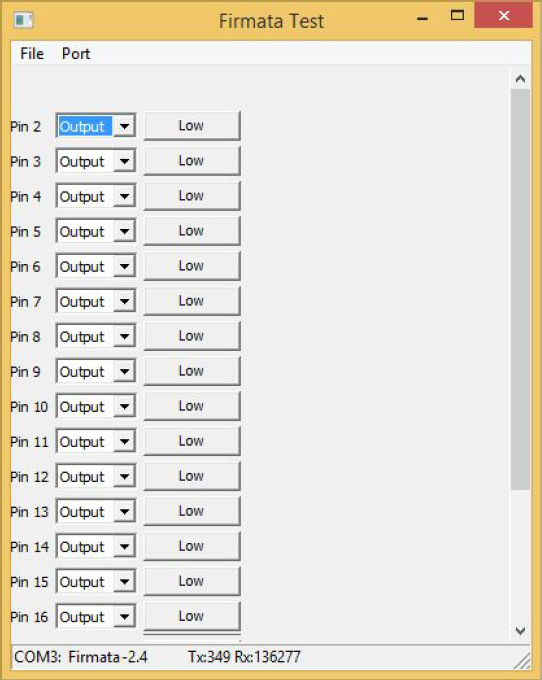
\includegraphics[width=12cm]{./Figures/firmataTest.png}
	\caption{Programa Firmata test}
	\label{fig:firmataTest}
\end{figure}

\begin{figure}[!htbp]
	\centering
	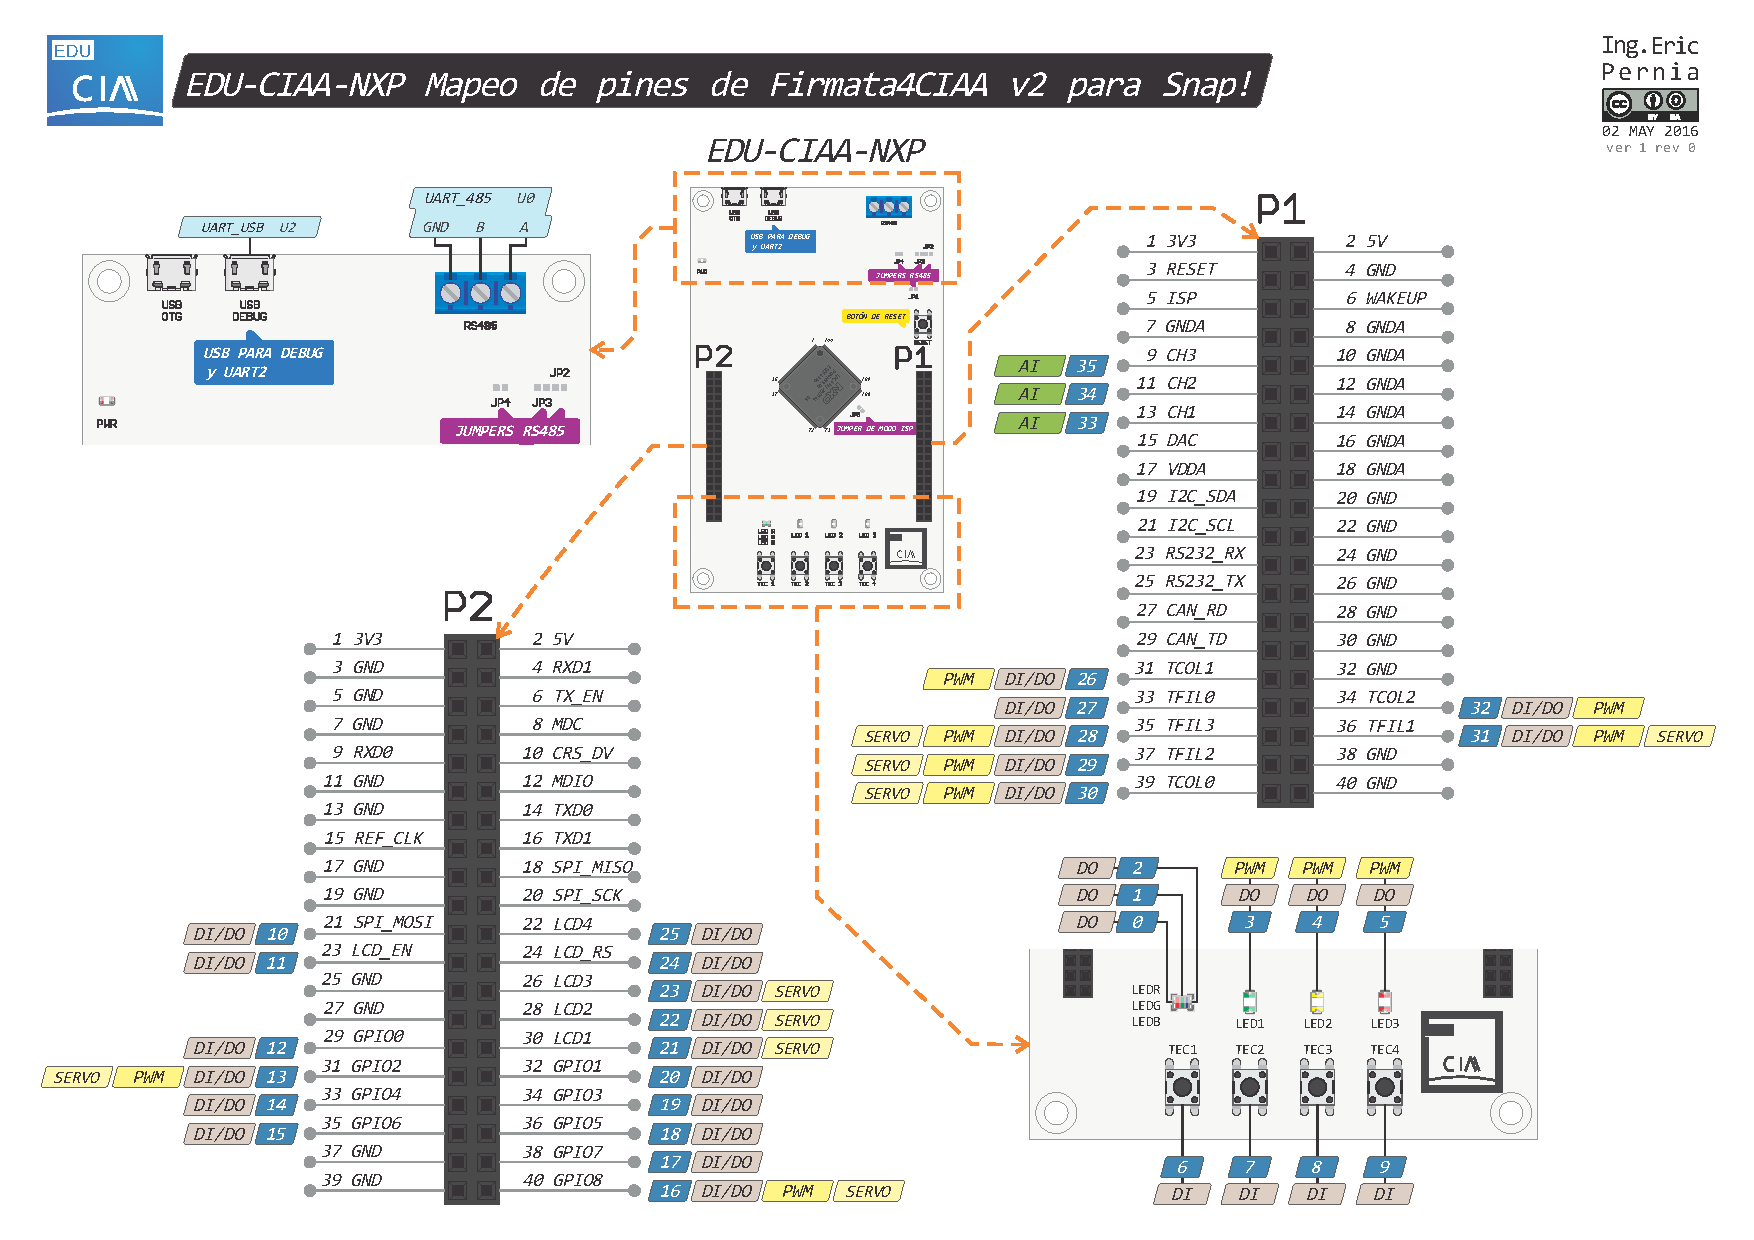
\includegraphics[width=12cm]{./Appendices/MapeoPinesFirmata4CIAAv2.pdf}
	\caption{Firmata4CIAA}
	\label{fig:MapeoPinesFirmata4CIAAv2}
\end{figure}

Para la verificación de Firmata de lado del cliente, se realizaron ensayos puntuales sobre la biblioteca \emph{Johnny five}. En la asignatura de Protocolos de Comunicación en Sistemas Embebidos de la CESE FIUBA \citep{CESE} se trabajo de forma puntual sobre el protocolo Firmata, realizando pruebas sobre un software web creado como trabajo final de la asignatura e instalado en la computadora, con el objetivo de ensayar todos los comandos del protocolo cliente sobre periféricos específicos conectados a la placa EDU-CIAA-NXP con Firmata4CIAA, y de esta manera realizar la manipulación de los mismos.  


\section{Ensayo de funcionamiento en los sistemas operativos Windows y Linux.}
\label{sec:Ensayo de funcionamiento en los sistemas operativos Windows y Linux.}

Este ensayo corresponde al “\emph{REQ1: El entorno de depuración deberá poder utilizarse dentro de los sistemas operativos Windows y Linux}”  y para llevarlo a cabo se realizaron los siguientes pruebas:

\subsection{Instalación en cada sistema.}
\label{subsec:Instalación en cada sistema.}

La instalación del sistema involucra la copia de los archivos necesarios para que el entorno de \emph{CIAABOT Debug} pueda funcionar sin problemas, en ambos sistemas operativos. 
Para llevar a cabo este \emph{test} se hizo la instalación en dos maquinas diferentes, una con el sistema operativo Windows y el otra con el sistema operativo Linux. 

El ensayo incluyó el proceso de descarga de los archivos del programa, y al ser exitosa, se ejecuto manualmente el siguiente \emph{test} funcional  sobre el estado \emph{Desconectado} para verificar de manera general el funcionamiento de \emph{CIAABOT Debug}. 

\subsubsection{\emph{Test} funcional posterior a la instalación en cada sistema}
Pre-condición:
\begin{itemize}
	\item \emph{CIAABOT Debug} se encuentra descargado en la computadora.
\end{itemize}
Flujo principal:
\begin{enumerate}
	\item
     Al Abrir \emph{CIAABOT Debug} se muestra al usuario la pantalla principal del entorno.
	\item
	El botón de inicio de sesión de depuración se muestra deshabilitado junto con las herramientas de control de ejecución.
	\item
	La edición de bloques del programa se encuentra habilitada.
\end{enumerate}

Resultado obtenido: en ambas computadoras se ejecutaron todos los pasos del \emph{test} sin problemas y de manera exitosa. 


\subsection{Chequeo de conexión y descarga de Firmata4CIAA.}
\label{subsec:Chequeo de acceso a puertos serie.}

Entre los archivos de \emph{CIAABOT Debug} se encuentra el archivo compilado que corresponde al proyecto de Firmata4CIAA  para la EDU-CIAA-NXP. Para proceder a la descarga de Firmata4CIAA, el entorno requiere que el usuario configure la ruta del \emph{toolchain} y de OpenOCD. Una vez realizado esto se comprobó mediante el siguiente \emph{test} manual la correcta comunicación entre el entorno, el \emph{toolchain} y \emph{openOCD}.

\subsubsection{\emph{Test} funcional descargar Firmata4CIAA}
Pre-condición:
\begin{itemize}
	\item
	\emph{CIAABOT Debug} se encuentra descargado en la computadora.
	\item
	La placa EDU-CIAA-NXP se encuentra conectada a la PC mediante el puerto marcado como \emph{USB Debug} en la serigrafía. La placa no tiene grabado el programa Firmata4CIAA.
\end{itemize}
Flujo principal:
\begin{enumerate}
	\item
	Al Abrir \emph{CIAABOT Debug} se muestra al usuario la pantalla principal del entorno.
	\item
    Al hacer click sobre el icono de configuración se muestra al usuario una ventana emergente para la configuración de los \emph{paths}.
	\item
	El usuario ingresa las rutas desde donde tiene el binario para el \emph{toolchain} y \emph{openOCD} y presiona el botón "Guardar".
	\item
	El usuario presiona el icono de actualizar desde la conexión con la plataforma.
	\item
	El entorno al estar en estado \emph{Conectado Sin Firmata4CIAA} consulta al usuario si quiere descargar Firmata4CIAA.
	\item
	El entorno avisa al usuario que la descarga fue exitosa.
\end{enumerate}

Resultado obtenido: en ambas computadoras se ejecutaron todos los pasos del \emph{test} sin problemas y de manera exitosa. 


\subsection{Chequeo de conexión con la plataforma EDU-CIAA-NXP.}
\label{subsec:Chequeo de conexión con la plataforma EDU-CIAA-NXP.}

El ensayo incluyó la comprobación del funcionamiento del inicio de la sesión de depuración para verificar que los bloques gráficos que acceden al hardware lo hagan de forma exitosa. Se ejecuto manualmente el siguiente \emph{test} funcional:

\subsubsection{\emph{Test} funcional de conexión con la plataforma EDU-CIAA-NXP}
Pre-condición:
\begin{itemize}
	\item
	\emph{CIAABOT Debug} se encuentra descargado en la computadora.
	\item
	La placa EDU-CIAA-NXP se encuentra conectada a la PC y con el programa Firmata4CIAA.
	\item
    El editor de programa de \emph{CIAABOT Debug} tiene importado un programa realizado en CIAABOT IDE.
\end{itemize}
Flujo principal:
\begin{enumerate}
	\item
	El programa de bloques se encuentra importado en el editor de programa de \emph{CIAABOT Debug}.
	\item
	Al usuario inicia la sesión de depuración haciendo click sobre el botón verde de \emph{debug}.
	\item
	El entorno habilita las herramientas de control de ejecución.
	\item
	El usuario hace click en el botón del icono \emph{ejecutar}.
	\item
	El entorno al detectar que existe un bloque gráfico con acceso a un periférico en particular, procede a realiza la conexión con la placa EDU-CIAA-NXP y muestra la manipulación del dispositivo al usuario.
\end{enumerate}

Resultado obtenido: en ambas computadoras se ejecutaron todos los pasos del \emph{test} sin problemas y de manera exitosa.



\section{Comprobación de funcionamiento de una sesión de depuración.}
\label{sec:Comprobación de funcionamiento de una sesión de depuración.}

Para poder verificar los siguientes requerimientos:

 \begin{itemize}
 	\item \emph{REQ2: Debe controlar de la ejecución de un programa corriendo en la plataforma de hardware}.
 	\item \emph{REQ3: Exponer el estado de las variables del programa en tiempo de ejecución}.
 \end{itemize}

 fueron necesarios realizar los siguientes ensayos de forma manual:

\subsection{Sesión de depuración uso del comando \emph{Ejecutar}}
Pre-condición:
\begin{itemize}
	\item \emph{CIAABOT Debug} se encuentra descargado en la PC.
	\item La placa EDU-CIAA-NXP se encuentra conectada a la PC y con el programa Firmata4CIAA.
	\item Existe un programa realizado en CIAABOT IDE con bloques gráficos de acceso al hardware.
\end{itemize}

Flujo principal:
\begin{enumerate}
	\item
	Al Abrir \emph{CIAABOT Debug} se muestra al usuario la pantalla principal del entorno. 
	\item
	El usuario elige el puerto serial desde donde tiene conectada la placa EDU-CIAA-NXP.
	\item
	El entorno detecta que la placa EDU-CIAA-NXP tiene descargado el programa Firmata4CIAA y habilita el inicio de sesión de depuración, mostrando el botón de \emph{debug} en color verde.
	\item
	El usuario presiona el botón verde de \emph{debug}.
	\item
	El entorno deshabilita la edición de programas, habilita las herramientas de control de ejecución y cambia el color del botón debug de verde a naranja.
	\item
	El usuario hace click en el botón de comando \emph{ejecutar}.
	\item
	El entorno ejecuta bloque por bloque el programa y al detectar que existe un bloque con acceso a un periférico envía la acción a la placa EDU-CIAA-NXP utilizando el protocolo firmata y muestra como salida la manipulación del dispositivo según lo programado por el usuario.
	\item
	El entorno actualiza el menú de visualización de variables con los nombres y valores de esas variables que se encuentran encastradas dentro de los bloques que están ejecutándose. 
\end{enumerate}

Resultado obtenido: ejecución de todos los pasos del \emph{test} en forma exitosa. 

\subsection{Sesión de depuración uso del comando \emph{Suspender}}
Pre-condición:
\begin{itemize}
	\item Sesión de depuración iniciada y programa en ejecución con el uso del comando \emph{ejecutar}.
\end{itemize}

Flujo principal:
\begin{enumerate}
	\item
	El entorno se encuentra ejecutando el programa con los bloques gráficos que acceden a periféricos como los que no acceden a periféricos.
	\item
	El usuario presiona el botón de \emph{suspender}.
	\item
	El entorno suspende la ejecución del programa, es decir, termina de ejecutar el bloque actual y se detiene antes del próximo bloque a ejecutar, el cual lo resalta con borde naranja.
	\item
	El usuario reanuda la ejecución del programa mediante el botón \emph{ejecutar}.
\end{enumerate}

Resultado obtenido: ejecución de todos los pasos del \emph{test} en forma exitosa.

\subsection{Sesión de depuración uso del comando \emph{Pasar por encima (step over)}}
Pre-condición:
\begin{itemize}
		\item Conexión con la plataforma establecida y la misma cuenta con Firmata4CIAA.
		\item Sesión de depuración iniciada. 
\end{itemize}

Flujo principal:
\begin{enumerate}
	\item
	El usuario hace click en el botón de comando \emph{Pasar por encima (step over)}.
	\item
	El entorno muestra resaltado el primer bloque del programa pero sin ejecutarlo.
	\item
	El usuario vuelve a hacer click en el botón de comando \emph{Pasar por encima (step over)}.
	\item
	El entorno muestra resaltado el bloque siguiente, ejecuta el bloque que fue resaltado anteriormente y actualiza el valor de las variables en el menú de visualizaciones de variables.
\end{enumerate}

Resultado obtenido: ejecución de todos los pasos del \emph{test} en forma exitosa.  

\subsection{Sesión de depuración uso del comando \emph{Pasar adentro (step into)}}
Pre-condición:
\begin{itemize}
	\item Conexión con la plataforma establecida y la misma cuenta con Firmata4CIAA.
	\item Sesión de depuración iniciada. 
\end{itemize}

Flujo principal:
\begin{enumerate}
	\item
	El usuario hace click en el botón de comando \emph{Pasar adentro (step into)}.
	\item
	El entorno muestra resaltado el primer bloque del programa pero sin ejecutarlo.
	\item
	El usuario vuelve a hacer click en el botón de comando \emph{Pasar adentro (step into)}.
	\item
	El entorno muestra resaltado el bloque siguiente, detecta que el bloque tiene un llamado a función y saltara a seleccionarlo. 
	\item
	El usuario vuelve a hacer click en el botón de comando \emph{Pasar adentro (step into)}.
	\item
	El entorno muestra resaltado el bloque siguiente dentro de la función y ejecutara el bloque anterior. 
\end{enumerate}

Resultado obtenido: ejecución de todos los pasos del \emph{test} en forma exitosa.  

\subsection{Sesión de depuración uso del comando \emph{Paso de regreso (step return)}}
Pre-condición:
\begin{itemize}
	\item Conexión con la plataforma establecida y la misma cuenta con Firmata4CIAA.
	\item Sesión de depuración iniciada y programa en ejecución con el uso del comando \emph{Pasar adentro (step into)}.
\end{itemize}

Flujo principal:
\begin{enumerate}
	\item
	El entorno se encuentra ejecutando el programa con los bloques gráficos resaltado los bloques con el uso del comando \emph{Pasar adentro (step into)} y ahora se encuentra dentro de una función.
	\item
	El usuario hace click en el botón de comando \emph{Paso de regreso (step return)}.
	\item
	El entorno ejecuta el bloque seleccionado y los siguientes sin seleccionarlos hasta encontrar el retorno de la función, luego seleccionara el siguiente bloque a continuación de la función que ejecuto.
\end{enumerate}

Resultado obtenido: ejecución de todos los pasos del \emph{test} en forma exitosa.  


\subsection{Sesión de depuración con puntos de ruptura (\emph{breakpoints})}
Pre-condición:
\begin{itemize}
     \item Sesión de depuración iniciada.
\end{itemize}

Flujo principal:
\begin{enumerate}
	\item
	El usuario hace \emph{click} con el botón derecho del \emph{mouse} en cualquiera de los bloques gráficos del programa.
	\item
	El entorno muestra el menú contextual del bloque desde donde se puede establecer el punto de interrupción.
	\item
	El usuario hace click dentro del menú contextual del bloque.
	\item
	El entorno establece el punto de interrupción en ese bloque, agrega un círculo rojo al mismo, en señal de \emph{breakpoint} y actualiza la ventana de visualización de puntos de ruptura con la información del nuevo \emph{breakpoint}.
	\item
	El usuario hace click en el botón del comando \emph{ejecutar}.
	\item
	El entorno ejecuta cada bloque de programa hasta llegar al bloque marcado con punto de interrupción donde detiene la ejecución y resalta el bloque con el \emph{breakpoint} que aún no ejecutó.
	\item
    El usuario hace click sobre el botón \emph{ejecutar}.
    \item
    El entorno continuará con la ejecución.
\end{enumerate}

Resultado obtenido: ejecución de todos los pasos del \emph{test} en forma exitosa. 


\subsection{Sesión de depuración uso del comando desactivar puntos de interrupción}
Pre-condición:
\begin{itemize}
	\item Sesión de depuración iniciada.
	\item Puntos de interrupción establecidos en algunos de los bloques.
\end{itemize}

Flujo principal:
\begin{enumerate}
	\item
	El usuario hace click en el botón de \emph{desactivar puntos de interrupción}.
	\item
	El entorno muestra el boton de \emph{desactivar puntos de interrupción} deshabilitado en señal de que se saltaran todos los puntos durante la ejecución  y actualiza el menú de visualización de puntos de ruptura (\emph{breakpoints}) mostrandolos desactivados.
	\item
	El usuario hace click en el botón del comando \emph{ejecutar}.
	\item
	El entorno resalta bloque por bloque el programa a medida que se va ejecutando sin detenerse al encontrar un punto de ruptura en el bloque establecidos anteriormente.
	\item
	El usuario hace click en el botón de \emph{desactivar puntos de interrupción}.
	\item
	El entorno muestra el botón de \emph{desactivar puntos de interrupción} habilitado y actualiza el menú de visualización de puntos de ruptura (\emph{breakpoints}) mostrandolos activados nuevamente.
\end{enumerate}

Resultado obtenido: ejecución de todos los pasos del \emph{test} en forma exitosa. 


\subsection{Sesión de depuración desactivar puntos de interrupción desde la ventana de visualización de \emph{breakpoints}}
Pre-condición:
\begin{itemize}
	\item Sesión de depuración iniciada.
	\item Puntos de interrupción establecidos en algunos de los bloques.
\end{itemize}

Flujo principal:
\begin{enumerate}
	\item
	El usuario hace click en uno de los \emph{checklist} actualmente tildado dentro del menú de visualización de puntos de ruptura (\emph{breakpoints}) de la columna “Activo”.
	\item
	El entorno muestra el \emph{checklist} destildado.
	\item
	El usuario hace click en el botón del comando \emph{ejecutar}.
	\item
	El entorno ejecuta los bloques de programa sin detenerse cuando encuentra el punto de ruptura en el bloque que fue destildado en la ventana de visualización de puntos de ruptura.
	\item
	El usuario hace click en el \emph{checklist} actualmente destildado dentro del menú de visualización de puntos de ruptura (\emph{breakpoints}) de la columna "Activo".
	\item
	El entorno ejecuta los bloques de programa y se detiene cuando encuentra el punto de ruptura en el bloque que fue tildado como activo desde la ventana de visualización de puntos de ruptura.
\end{enumerate}

Resultado obtenido: ejecución de todos los pasos del \emph{test} en forma exitosa. 


\subsection{Sesión de depuración uso del comando \emph{Detener depuración}}
Pre-condición:
\begin{itemize}
	\item Conexión con la plataforma establecida y la misma cuenta con firmata.
\end{itemize}

Flujo principal:
\begin{enumerate}
	\item
El entorno se encuentra con una sesión de depuración iniciada (se comprueban los casos con sesión en ejecución y con sesión de suspensión en ejecución).
	\item
	El usuario presiona el botón de \emph{detener depuración}.
	\item
	El entorno termina la ejecución del programa, finaliza la sesión de depuración, cambia el botón de \emph{debug} de color naranja a color verde y por ultimo habilita la edición del programa.
\end{enumerate}

Resultado obtenido: ejecución de todos los pasos del \emph{test} en forma exitosa. 

\subsection{Guardado y restauración de los puntos de ruptura}
Pre-condición:
\begin{itemize}
	\item \emph{CIAABOT Debug} se encuentra descargado en la PC.
    \item La placa EDU-CIAA-NXP se encuentra conectada a la PC y con el programa Firmata4CIAA.
    \item Existe un programa realizado en CIAABOT IDE y abierto en el editor de programas del entorno de \emph{debug}.
    \item Sesión de depuración iniciada.
\end{itemize}

Flujo principal:
\begin{enumerate}
    \item
	El usuario hace click derecho en cualquiera de los bloques gráficos que se muestran dentro del editor.
	\item
	El entorno muestra el menú contextual del bloque desde donde se puede establecer el punto de interrupción.
	\item
	El usuario hace click dentro del menú contextual del bloque.
	\item
	El entorno establece el punto de interrupción en ese bloque, agrega un punto rojo en señal de \emph{breakpoint} y actualiza la ventana de visualización de puntos de ruptura con la información del nuevo \emph{breakpoint}.
	\item
	El usuario hace click en el botón del comando \emph{ejecutar}.
	\item
	El entorno ejecuta los bloques de programa.
	\item
    El usuario detiene la sesión de depuración y cierra el programa, o abre otro programa.
	\item
	El entorno actualiza el archivo debug.cbd. dentro de la carpeta que contiene el proyecto automáticamente.
	\item
	El usuario hace click nuevamente en el menú "Proyecto" de la aplicación y abre el proyecto usado previamente  en el punto anterior.
	\item
	El entorno carga nuevamente el programa en el editor de \emph{debug}.
	\item
	El usuario comprueba que el punto de interrupción establecido anteriormente para ese bloque aparece nuevamente en el editor.
	
\end{enumerate}

Resultado obtenido: ejecución de todos los pasos del \emph{test} en forma exitosa. 


\section{Ensayos de edición de programas en lenguaje CIAABOT.}
\label{sec:Ensayos de edición de programas en lenguaje CIAABOT.}

Para poder verificar el requerimiento “\emph{REQ4: Permitir la edición de programas para corregir errores de lógica encontrados en tiempo de ejecución}”
fue necesario realizar el siguiente ensayo de forma manual:

\subsection{Edición de programa}
Pre-condición:
\begin{itemize}
	\item \emph{CIAABOT Debug} se encuentra descargado en la PC.
	\item La placa EDU-CIAA-NXP se encuentra conectada a la PC y con el programa Firmata4CIAA.
	\item Existe un programa realizado en CIAABOT IDE.
\end{itemize}

Flujo principal:
\begin{enumerate}
	\item
	Al Abrir \emph{CIAABOT Debug} se muestra al usuario la pantalla principal del entorno.
	\item
	El usuario elige el puerto serial desde donde tiene conectada la placa EDU-CIAA-NXP.
	\item
	El entorno detecta que la placa EDU-CIAA-NXP tiene descargado el programa Firmata4CIAA y habilita el inicio de sesión de depuración, mostrando el botón de \emph{debug} en color verde.
	\item
	El usuario realiza la modificación de los bloques gráficos, para ello agrega un nuevo bloque a la estructura de bloques del programa y guarda el programa actualizado desde el menú "Proyecto" de la aplicación.
	\item
	El entorno guarda el programa actualizado y actualiza el archivo .cbp dentro de la carpeta que contiene el proyecto guardado.
	\item
	El usuario hace click en el menú "Proyecto" de la aplicación y abre el proyecto que fue guardado en el punto anterior.
	\item
	El entorno carga nuevamente el programa en el editor de \emph{debug}.
	\item
	El usuario comprueba que el bloque gráfico agregado en el punto anterior se encuentre en el programa cargado.
\end{enumerate}

Resultado obtenido: ejecución de todos los pasos del \emph{test} en forma exitosa.


\section{Ensayos de interfaz de usuario.}
\label{sec:Ensayos de interfaz de usuario.}

Para poder verificar los requerimientos:
\begin{itemize}
	\item \emph{REQ5: La interfaz gráfica debe seguir los lineamientos de estilo establecidos en el Proyecto CIAABOT}.
	\item \emph{REQ6: Debe presentar un diseño de interfaz gráfica intuitiva, con elementos similares a los hallados en otras herramientas de depuración}.
\end{itemize}

Como parte de la verificación en los estilos visuales del diseño de la interfaz del entorno de \emph{debug} se realizaron reuniones con el director de este trabajo y con especialistas en diseño de interfaz de usuario para la evaluación de prototipos html, con la intención de descubrir errores en el funcionamiento que no cumplan los requerimientos, y ademas el de tener presente los posibles problemas de uso que podrían tener los usuarios.


\section{Validación con usuarios.}
\label{sec:Validación con usuarios.}

Para verificar el requerimiento “\emph{REQ6: Debe presentar un diseño de interfaz gráfica intuitiva, con elementos similares a los hallados en otras herramientas de depuración}” se realizaron ensayos de los usuarios finales en el marco de un laboratorio de programación llevado a cabo en la materia “\emph{Computadores 2 / Técnicas Avanzadas de Programación UNQ 2018}” \citep{computadores2unq2018} de la Universidad nacional de Quilmes. Los usuarios con experiencia de depuración en lenguaje C pudieron utilizar el entorno sin necesidad de algún soporte en la utilización de la herramienta de comandos para depuración que ofrece la plataforma, siendo esto prueba que el diseño de interfaz gráfica es intuitiva y de fácil uso. 
% Chapter Template

\chapter{Conclusiones} % Main chapter title

\label{Chapter5} % Change X to a consecutive number; for referencing this chapter elsewhere, use \ref{ChapterX}


%----------------------------------------------------------------------------------------

%----------------------------------------------------------------------------------------
%	SECTION 1
%----------------------------------------------------------------------------------------

\section{Conclusiones generales }

En el presente Trabajo Final se ha logrado obtener un entorno de depuración para la plataforma CIAABOT. El entorno de depuración \emph{ CIAABOT Debug} otorga una interfaz simple e intuitiva para depurar programas en lenguaje CIAABOT, utilizando la plataforma EDU-CIAA-NXP.

En el desarrollo de este Trabajo Final se aplicaron los conocimientos adquiridos en la Carrera de Especialización en Sistemas Embebidos, en especial las asignaturas:

\begin{itemize}
	\item Programación de microprocesadores. En esta materia se aprendió a utilizar la EDU-CIAA-NXP y herramientas de depuración en lenguaje C. Estas herramientas permitieron entender como se utiliza la depuración de un sistema embebido desde la PC.
	\item Ingeniería de software en sistemas embebidos. Se utilizaron técnicas y metodologías de trabajo de la ingeniería del software. Se usaron los conocimientos de manejo de repositorio Git como sistema de control de versiones y se aplicaron metodologías de ensayo de software.
	\item Gestión de Proyectos en Ingeniería. Plan de Proyecto para organizar el Trabajo Final, permitió desde el inicio de la carrera tener una visión de todas las tareas a realizar y su estimación en tiempos.
	\item Protocolos de Comunicación. Se aplicaron los conocimientos obtenidos del protocolo Firmata.
	\item Sistemas Operativos de Propósito General. Se usaron los conocimientos sobre Linux, usando las herramientas que provee para usarse en las pruebas generales del software creado.
\end{itemize}


El entorno de \emph{CIAABOT debug} le da la capacidad de depuración al proyecto CIAABOT, por lo tanto tambien aporta al Proyecto CIAA, y a la comunidad de sistemas embebidos en general.

Se concluye que los objetivos del trabajo han sido cumplidos satisfactoriamente, se logró un mejor conocimiento del hardware y el desarrollo del mismo ha favorecido en
gran medida a la formación profesional de la autora.


%----------------------------------------------------------------------------------------
%	SECTION 2
%----------------------------------------------------------------------------------------
\section{Próximos pasos}

Se propone agregar las siguientes características al entorno de depuración:

\begin{itemize}
	\item Capacidad de evaluación de expresiones.
	\item Ver \emph{stack} de llamadas a funciones.
	\item Consola de comandos del \emph{debug}.
\end{itemize}
 

%----------------------------------------------------------------------------------------
%	CONTENIDO DE LA MEMORIA  - APÉNDICES
%----------------------------------------------------------------------------------------

\appendix % indicativo para indicarle a LaTeX los siguientes "capítulos" son apéndices

% Incluir los apéndices de la memoria como archivos separadas desde la carpeta Appendices
% Descomentar las líneas a medida que se escriben los apéndices

%% Appendix A

\chapter{Appendix Title Here} % Main appendix title

\label{AppendixA} % For referencing this appendix elsewhere, use \ref{AppendixA}

Write your Appendix content here.
%\include{Appendices/AppendixB}
%\include{Appendices/AppendixC}

%----------------------------------------------------------------------------------------
%	BIBLIOGRAPHY
%----------------------------------------------------------------------------------------

\Urlmuskip=0mu plus 1mu\relax
\raggedright
\printbibliography[heading=bibintoc]

%----------------------------------------------------------------------------------------

\end{document}  
